\documentclass[tc, manuscript]{copernicus}

\usepackage{appendix}

% check if we are compiling under latex or pdflatex
%\ifx\pdftexversion\undefined
%\usepackage[dvips]{graphicx}
%\else
%\usepackage[pdftex]{graphicx}
%\usepackage{epstopdf}
%\epstopdfsetup{suffix=}
%\fi

% the default is for unnumbered section heads
% if you really must have numbered sections, remove
% the % from the beginning of the following command
% and insert the level of sections you wish to be
% numbered (up to 4):

% \setcounter{secnumdepth}{2}

\begin{document}
\title{Diagnosising the sensitivity of grounding line flux to changes in sub-ice shelf melting}

\Author[1]{Tong}{Zhang}
\Author[1]{Stephen}{Price}
\Author[1]{Matthew}{Hoffman}
\Author[2]{Mauro}{Perego}
\Author[1]{Xylar}{Asay-Davis}

\affil[1]{Fluid Dynamics and Solid Mechanics Group, Los Alamos National Laboratory, Los Alamos, NM, 87545, USA}
\affil[2]{Center for Computing Research, Sandia National Laboratories, Albuquerque, NM, 87185, USA}

\runningtitle{Diagnosising the sensitivity of grounding line flux to sub-ice shelf melting}
\runningauthor{T.~Zhang et al.}
\correspondence{T.~Zhang (tzhang@lanl.gov)}

\received{}
\pubdiscuss{} %% only important for two-stage journals
\revised{}
\accepted{}
\published{}

\firstpage{1}
\maketitle
 
\begin{abstract}
In this paper, we look for an improved physical understanding for how ice dynamics link ice thickness perturbations, via changes in sub-ice shelf melting, to changes in ice shelf buttressing and grounding line flux. More specifically, we seek a connection among grounding line flux, ice shelf buttressing and basal melting. By studying the ice dynamics for both idealized (MISMIP+) and realistic (Larsen C) ice shelves, we find a strongly direction-dependent buttressing number that links local changes in ice shelf thickness and dynamics with changes in the integrated grounding line flux. From these two examples, this buttressing metric, defined using the first principal stress, is better overall for quantifying changes in grounding line flux than a similar metric defined using the second principal stress or stress along the flow direction. This correlation is possibly controlled by the relative relationship of geometric/dynamic features between the perturbation point and the grounding line, indicating a dynamic (time evolving) sensitivity field of integrated grounding line flux to basal melt. We find this buttressing metric only shows a robust relationship with the integrated grounding line flux for regions near the center of an ice shelf; for points too near the grounding line or the calving front, no clear relationship exists. This motivates our exploration of an adjoint-based method for defining integrated grounding line flux sensitivity to local changes in ice shelf geometry. \textbf{TZ: add 1-2 sentences describing the results of adjoint when we get the larsen C results, for example, what does adjoint look like near GL?}
\end{abstract}

%\copyrightstatement{TEXT}



\introduction

Marine ice sheets like West Antarctica (and to a lesser extent, portions of East Antarctica) are grounded below sea level and their bedrock would remain so even after full isostatic rebound \citep{barletta2018}. This and the fact that ice sheets generally thicken inland lead to a geometric configuration that are prone to instability; a small increase in flux at the grounding line thins the ice there, leading to floatation, a retreat of the grounding line into deeper water, further increases in flux (due to still thicker ice), and further thinning and grounding line retreat. This theoretical ``marine ice sheet instability'' mechanism \citep{mercer1978, schoof2007} is supported by idealized \citep[e.g.,][]{schoof2012, asay2016} and realistic \citep[e.g.,][]{Cornford2015,royston2016} ice sheet modeling experiments and some studies \citep{joughin2014,rignot2014} argue that such an instability is currently under way along outlet glaciers of Antarctica's Amundsen Sea Embayment (ASE). The relevant perturbation for grounding line retreat in the ASE is thought to be intrusions of relatively warm, intermediate-depth ocean waters onto the continental shelves, which have reduced the thickness and extent of marginal ice shelves via increased submarine melting \citep[e.g.,][]{JenkinsEtAl2016}. These reductions are critical because fringing ice shelves restrict the flux of ice across their grounding lines farther upstream---the so-called ``buttressing'' affect of ice shelves \citep{gudmundsson2012, gudmundsson2013, derydt2015}---which makes them a critical control on the rate of ice flux from Antarctica to the ocean.

%It is therefore a big concern at present if the marine-type West Antarctica Ice Sheet (WAIS) will accelerately retreat and cause a significant sea level rise in the near future \citep{joughin2011}. As ice shelves can supply additional resisting forces (buttressing) to ice flow from upstream and thus decrease the ice flux across grounding line (GL), they are critical for stabilizing marine ice sheets from further retreating \citep{gudmundsson2013}. 

%Warm ocean water is getting more evident of being responsible of increased melt at the base of ice shelves in Antarctica \citep{jenkins2018,rintoul2016}. The basal melting decreases ice thickness and reduce the buttressing ability of ice shelf \citep{gagliardini2010}, and can therefore potentially destabilize marine ice sheets. Satellite altimetry measurements have proved this mechanism that ice shelf thickness decrease links glacier acceleration in Antarctica \citep{pritchard2012}. Recent studies also suggested that the thinning of ice shelfves also contributes to the ice dynamic changes of upstream grounded ice sheets \citep{minchew2018}, indicating the importance of ice shelf-ocean coupling in the whole ice sheet dynamics. 
On ice shelves, gradients in hydrostatic pressure are balanced primarily by the extensional flow of ice towards the calving front \citep{hutter1983, morland1987, schoof2007} and, in theory, an ice shelf in one horizontal dimension ($x$-$z$) provides no buttressing \citep{schoof2007,gudmundsson2013}. For realistic, three-dimensional ice shelves however,  buttressing results from three main sources: 1) compressive ice flow, 2) lateral shear, and 3) ``hoop'' stress \citep{pegler2012}. Both compressive and lateral shear stresses can supply backward resistance to extensional ice shelf flow through along-flow and across-flow stress gradients, while hoop stress is a transverse stress arising from azimuthal extension in regions of diverging flow \citep{wearing2016}.  Due to the complex geometries, kinematics, and dynamics of real ice shelves, an understanding of the specific processes and locations that control ice shelf buttressing is far from straightforward.

Several recent studies apply whole-Antarctic ice sheet models, optimized to present-day observations, towards improving our understanding for how Antarctic ice shelves limit flux across the grounding line (and by extension how they impact ice dynamics farther inland). \citet{furst2016} calculated the buttressing number across Antarctica ice shelves along two major directions (aligned with the ice flow and with the second principal stress) and evaluated their impacts on upstream ice dynamics to identify regions of the ice shelves that are dynamically ``passive''; in these regions increased submarine melting, or even complete removal of the ice should not significantly alter local or regional ice dynamics or the flux of from ice upstream. \citet{reese2018} used perturbation experiments to link small, localized decreases in ice shelf thickness to changes in integrated grounding line flux (GLF), thereby providing a map of GLF sensitivity to local increases in submarine melt rates. \citet{Goldberg2019} assessed the consistency of satellite retrieved and modeled melt rates, found the importance of bathymetry in influencing the ice sheet responses predicted by models and also investigated the adjoint sensitivity of volume above floatation to melt rates for Dotson and Crosson ice shelves, Antarctica.


%SP: After writing this sentence, it occurs to me that something else that we could follow up on at some point is if / how broader patterns of ice thickness change might complicate the interpretation of these simple perturbation experiments. E.g., you can imagine that 1) multiple perturbations in diff. areas of the ice shelf might conflict with one another and have a more complex impact on g.l. flux (e.g., simultaneous perturbations in multiple areas that show both g.l. flux increases and decreases w/ ice thickness perturbations), 2) similar scale perturbations but applied over wider areas (e.g., over an area that is representative of the actual length scale of submarine melt patterns). Maybe this would be implicit in any 2nd or later study where we perturbed ice shelves based on the sensitivity maps we derive from the adjoint method.

%TZ: Yes. This is what I've been thinking of for a while. What I am not quite sure is how we design such complex (but also follow some simplied patterns) perturbation conflicts? Is there anything we can borrow from the ocean modeling results (e.g. ALCC)?

\textbf{Steve to update this paragraph to better reflect what we actually do below: 1) connect the studies of Furst and Reese by trying to understand if / how local evaluations of ice shelf buttressing do or do not reflect the actual potential for purturbations at those same locations to impact the flux across the GL (since that is, presumably, why we care about buttressing in the first place -- noting that what we'd like is some easily calculated 'metric' to identify these important locations for us); 2) assess the ability of analagous, relatively easy to calculate, local buttressing metrics to indicate GLF sensitivity to local perturbations in ice shelf geometry; 3) point out where these metrics are useful and where (and why) they are not; 4) propose and demonstrate alternate, adjoint-based method that has advantages over previous methods.}
Motivated by these studies, we build on and extend the methods and analysis of \citet{furst2016} and \citet{reese2018} in order to make progress towards answering the following questions: 
(1) Is there any easily accessible metrics that indicate the sensitivity of GLF to the thickness change at certain locations on ice shelf?
(2) Is buttressing number a such metric? Does thickness decrease at the locations with large buttressing number results in large GLF increase?
(3) What are the mechanisms that connect ice thickness perturbation (basal melting) and GLF changes?
%(1) How do local and regional changes in ice shelf geometry affect distal changes in GLF? 
%(2) Can local or regional ice shelf dynamics explain GLF sensitivity to local or regional changes in ice shelf thickness? 
(4) Can we derive easy-to-implement and new methods/metrics for indicating the GLF sensitivity of basal melting across ice shelf during the model run over time so that we can better project how changes in submarine melt pattern and magnitude will impact GLF in the future?  

% OLDER: In this study we aim to further improve the understanding of how changes in submarine melting impact grounding line flux, and by inference, marine ice sheet stability. Using both idealized  (MISMIP+; Fig \ref{mismip_larsenc}a) and realistic (Larsen C; Fig \ref{mismip_larsenc}b) ice shelf geometries, we conduct model perturbation experiments similar to those of \citet{reese2018}. Our goal is to better understand the ice dynamical processes linking a local perturbation in ice shelf thickness (via submarine melt changes) to a change in grounding line flux. \textit{SP: I'm not sure if we actually do contribute much to this understanding though, so we might need to refocus this depending on what we actually include in the final version of the paper.} In addition, we explore diagnostics for quantifying grounding-line-flux sensitivity as a function of changes in submarine melt with an eye towards defining quantitative sensitivity ``metrics'' that are readily calculated from standard ice sheet model outputs. 

Below, we first provide a brief description of the ice sheet model used in our study. We follow with a description of the model experiments. We then demonstrate and discuss the experimental results, including defining metrics for quantifying GLF sensitivity to changes in submarine melt, explaining their origins, and exploring their applicability and limitations.  We conclude by proposing and demonstrating an adjoint-based calculation that provides a sensitivity map analogous to the perturbation experiments from \citet{reese2018} but at the cost of a single adjoint solve in the model. 

%\textbf{TZ: the Goldberg 2019 paper has already mentioned the adjoint method...Not sure yet how to revise it to avoid conflicts with their conclusions. SP: Agreed - that's why I thought we needed to mention it. But even if their application is similar, it's still fair game for us to introduce it here (we are pointing out the connection between that and Reese et al., which they do not do) as long as we acknowledge their work.}

\begin{figure}
\centering
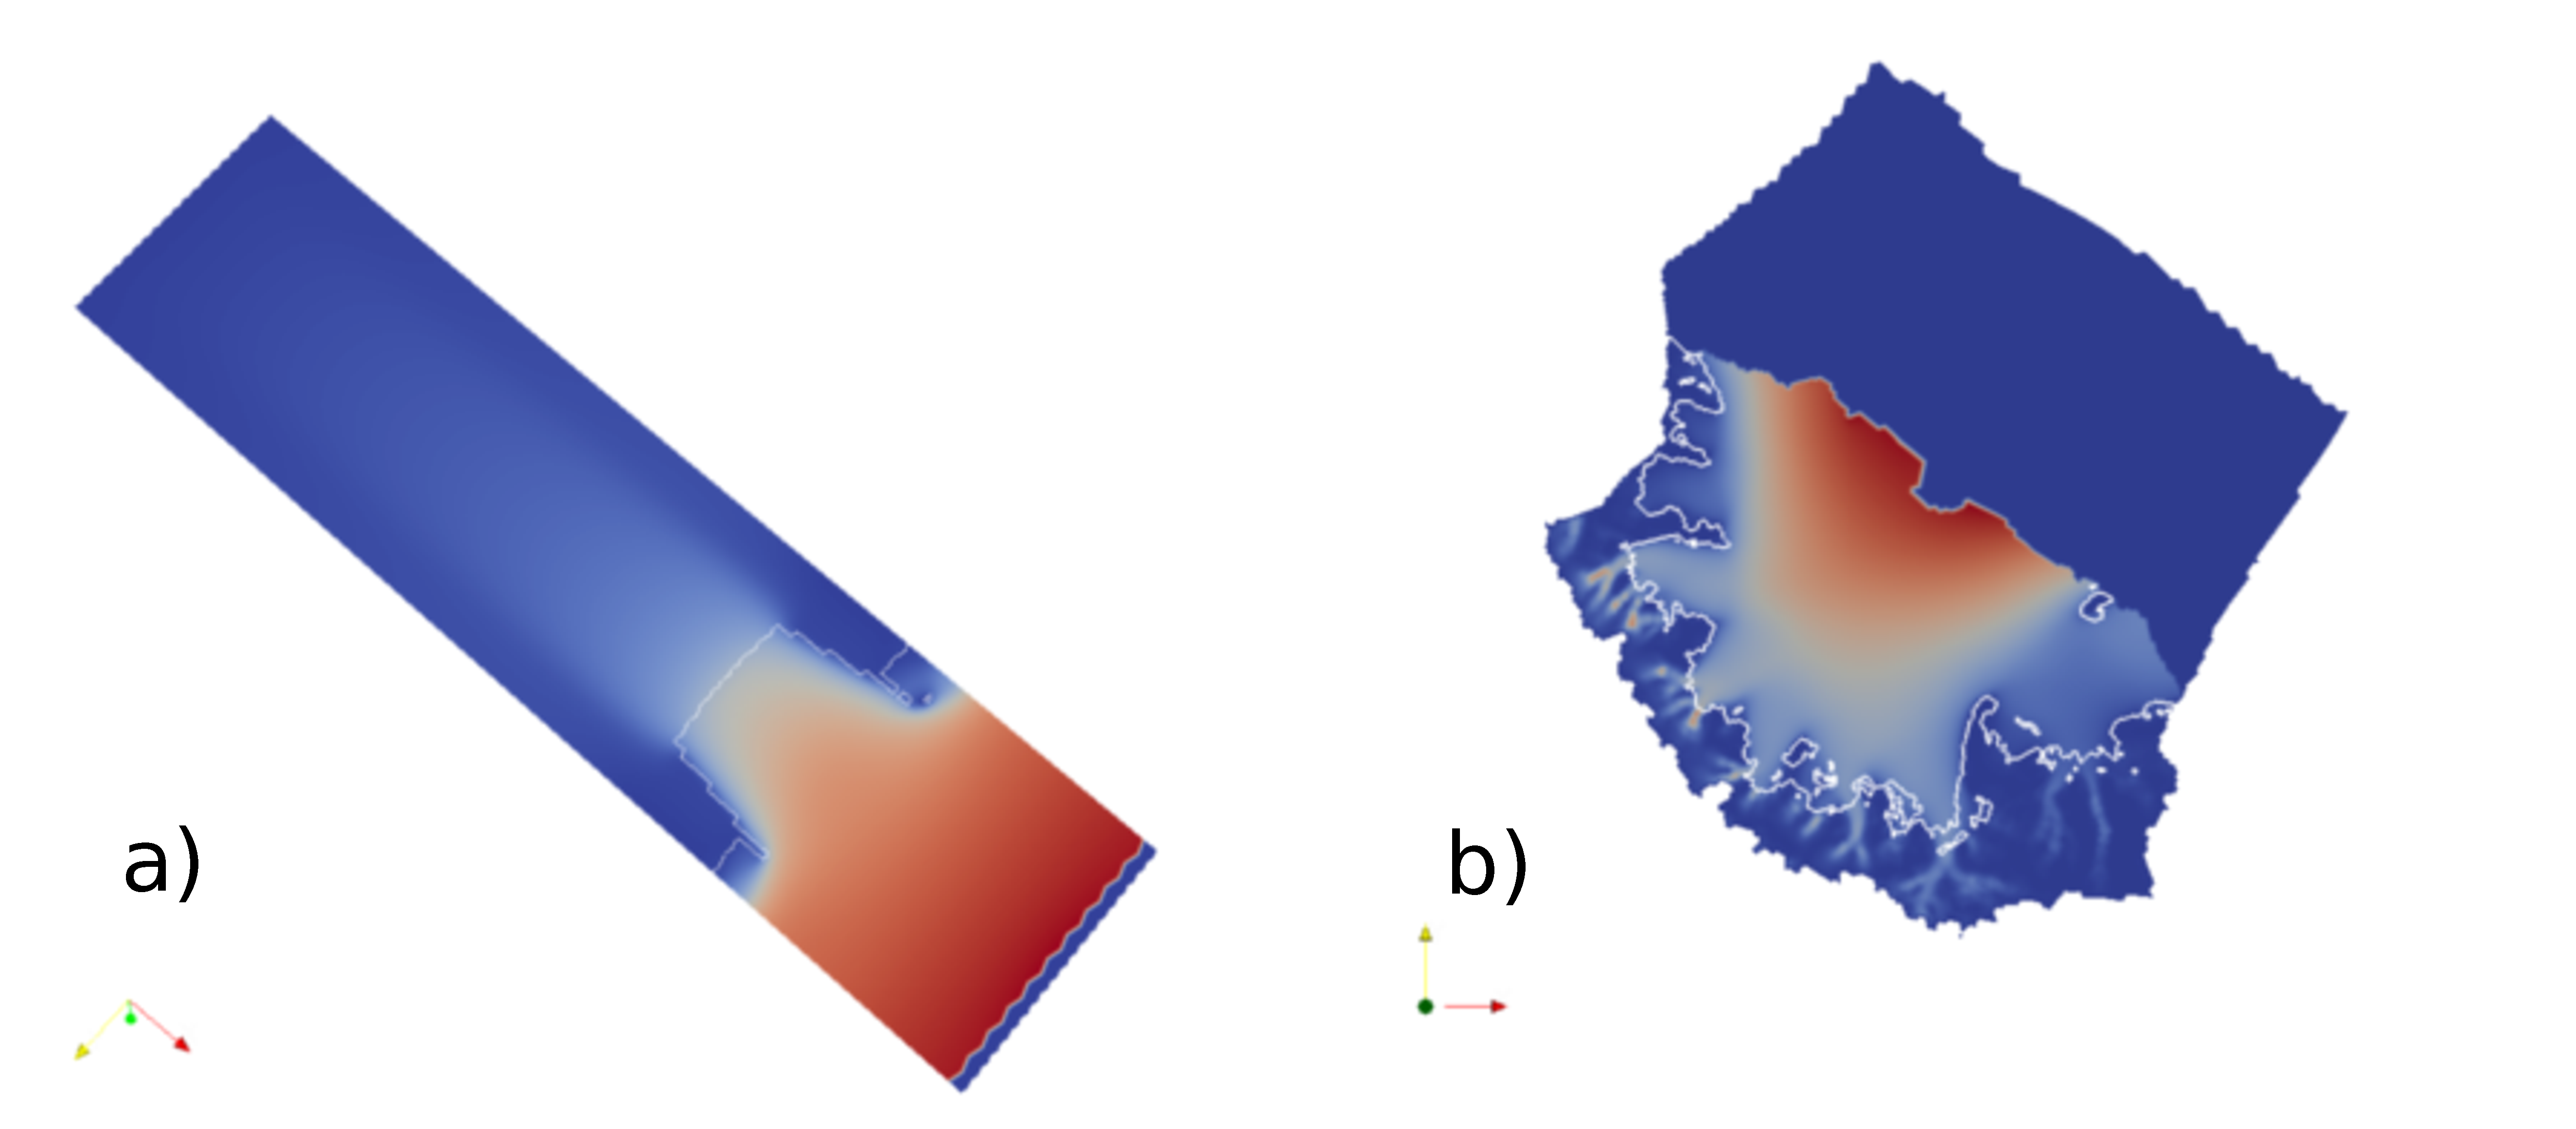
\includegraphics[width=1\linewidth]{./figs/mismip_larsenc.pdf}
\caption{Plan view of steady-state surface speed for a) MISMIP+ and b) Larsen C Ice Shelf. The black curves show the grounding lines.}
\label{mismip_larsenc}
\end{figure}

\section{Model description}
We use the MPAS-Albany Land Ice model \citep[MALI;][]{hoffman2018}, which solves the three-dimensional, first-order approximation to the Stokes momentum balance for ice flow\footnote{See \citet{schoof2013} for a full description of the Stokes momentum balance for ice flow and its lower-order approximations.}. Using the notation  of \citet{perego2012} and \citet{tezaur2015a} this can be expressed as, 
\begin{equation} \label{eq:foStokes}
\left\{
\begin{array}{rcl} -\nabla \cdot (2 \mu_e \dot{\boldsymbol{\epsilon}}_1) + \rho_{i} g
\frac{\partial s}{\partial x}&=&0, \\
-\nabla \cdot (2 \mu_e \dot{\boldsymbol{\epsilon}}_2) +\rho_{i} g
\frac{\partial s}{\partial y} &=& 0, \\
\end{array}\right.
\end{equation}
where $x$ and $y$ are the horizontal coordinate vectors in a Cartesian reference frame, $s(x,y)$ is the ice surface elevation, $\rho_{i}$ represents the ice density, $g$ the acceleration due to gravity, and $\dot{\boldsymbol{\epsilon}}_{1,2}$ are the two dimensional strain rate vectors given by
\begin{equation}
\dot{\boldsymbol{\epsilon}}_1 = \left(\begin{array}{ccc}
2\dot{\epsilon}_{xx} + \dot{\epsilon}_{yy}, &\dot{\epsilon}_{xy},&
\dot{\epsilon}_{xz}\end{array}\right)^T,
\end{equation}
and
\begin{equation}
\dot{\boldsymbol{\epsilon}}_2 = \left(
\begin{array}{ccc}\dot{\epsilon}_{xy}, &
\dot{\epsilon}_{xx} + 2\dot{\epsilon}_{yy}, &\dot{\epsilon}_{yz}
\end{array}\right)^T.
\end{equation}
The ``effective'' ice viscosity, $ \mu_e$ in  Eq.~(\ref{eq:foStokes}), is given by 
\begin{equation}
\label{eq:effvisc}
    \mu_{e}~=~\gamma A^{-\frac{1}{n}}\dot{\epsilon}_{e}^{\frac{1-n}{n}},
\end{equation}
where $\gamma$ is an ice stiffness factor, $A$ is a temperature-dependent rate factor, $n=3$ is the power-law exponent, and the effective strain rate, $\dot{\epsilon}_{e}$, is defined as
\begin{equation} \label{eq:effstrain}
\dot{\epsilon}_e \equiv \left( \dot{\epsilon}_{xx}^2 +
\dot{\epsilon}_{yy}^2 + \dot{\epsilon}_{xx} \dot{\epsilon}_{yy} +
\dot{\epsilon}_{xy}^2 + \dot{\epsilon}_{xz}^2 +
\dot{\epsilon}_{yz}^2 \right)^\frac{1}{2},
\end{equation}
where $\dot{\epsilon}_{ij}$ are the corresponding strain-rate components.
%Gradients in the horizontal velocity components, $u$ and $v$, contribute to the individual strain rate terms in (\ref{eq:effstrain}) and are given by
%\begin{eqnarray} \label{eq:epsilonij}
%\dot{\epsilon}_{xx} &=& \frac{\partial u}{\partial x}, \hspace{0.5cm} 
%\dot{\epsilon}_{yy} = \frac{\partial v}{\partial y}, \hspace{0.5cm}
%\dot{\epsilon}_{xy} = \frac{1}{2}\left(\frac{\partial u}{\partial y} + \frac{\partial v}{\partial x} \right), \nonumber\\ 
%\dot{\epsilon}_{xz} &=& \frac{1}{2} \frac{\partial u}{\partial z}, \textrm{ and } \hspace{0.15cm} 
%\dot{\epsilon}_{yz} = \frac{1}{2} \frac{\partial v}{\partial z}.
%\end{eqnarray}

A stress free upper surface is enforced through 
\begin{equation} \label{eq:stressFreeBC}
\dot{\boldsymbol{\epsilon}}_1 \cdot \mathbf{n} = \dot{\boldsymbol{\epsilon}}_2 \cdot \mathbf{n} = 0, 
\end{equation}
%\begin{equation} \label{eq:stressFreeBC}
%\boldsymbol{\sigma} \cdot \mathbf{n} = 0, 
%\end{equation}
where $\mathbf{n}$ is the outward pointing normal vector at the ice sheet upper surface, $z=s(x,y)$.
The lower surface is allowed to slide according to the continuity of basal tractions,
\begin{equation} \label{eq:basalbc}
\begin{array}{ll}
2\mu_e \dot{\boldsymbol{\epsilon}}_1 \cdot \mathbf{n} + \beta u = 0, \hspace{0.2cm} 2 \mu \dot{\boldsymbol{\epsilon}}_2 \cdot \mathbf{n} + \beta v = 0, \\
\end{array}
\end{equation}
%\begin{equation} \label{eq:basalbc}
%\boldsymbol{\sigma} \cdot \mathbf{n} + \beta \boldsymbol{u} = 0,
%\end{equation}
where $\beta$ is a spatially variable friction coefficient, $\boldsymbol{\sigma}$ is the stress tensor and $\boldsymbol{u}$ is the two-dimensional velocity vector ($u$, $v$). On lateral boundaries in contact with the ocean, the portion of the boundary above sea level is stress free while the portion below sea level feels the ocean hydrostatic pressure according to
\begin{equation}\label{eq:oceanbc}
\begin{array}{ll}
2 \mu_e \dot{\boldsymbol{\epsilon}}_1 \cdot \mathbf{n} = \frac{1}{2} \rho_i g H \left(1- \frac{\rho_i}{\rho_o} \right) \mathbf{n}_1, \quad 2 \mu_e  \dot{\boldsymbol{\epsilon}}_2 \cdot \mathbf{n} = \frac{1}{2} \rho_i g H \left(1- \frac{\rho_i}{\rho_o} \right) \mathbf{n}_2
\end{array}
\end{equation}
%\begin{equation}\label{eq:oceanbc}
%\boldsymbol{\sigma} \cdot \mathbf{n} = \rho_i g (s-z)\mathbf{n},
%\end{equation}
%where $\rho_o$ represents the density of ocean water and $xx\mathbf{n}$ the outward pointing normal vector to the lateral boundary (i.e., parallel to the $(x,y)$ plane).
where $\mathbf{n}$ is the outward pointing normal vector to the lateral boundary (i.e., parallel to the $(x,y)$ plane) and $\rho_o$ is the density of ocean water.
%\textbf{TZ: I change this section a bit to avoid it looking identical to Matt's MALI paper.}

A more complete description of the MALI model, including the implementations for mass and energy conservation, can be found in \citet{hoffman2018}. Additional details about the Albany momentum balance solver can be found in \citet{tezaur2015a,tezaur2015b}. 

Here, we apply MALI to experiments on both idealized and realistic marine-ice sheet geometries. For our idealized domain and model state, we start from the equilibrium initial conditions for the MISMIP+ experiments, as described in \citet{asay2016}. The model mesh is spatially uniform at an around 2 km resolution. For our realistic domain, we use Antarctica's Larsen C Ice Shelf and its upstream catchment area. The model state is based on the optimization of the ice stiffness ($\gamma$ in Eq. (\ref{eq:effvisc})) and basal friction ($\beta$ in Eq. (\ref{eq:basalbc})) coefficients in order to provide a best match between modeled and observed present-day velocities \citep{rignot2014} using adjoint-based methods discussed in \citet{perego2014} and \citet{hoffman2018}. The domain geometry is based on Bedmap2 \citep{fretwell2013} and ice temperatures, which are held fixed for this study, are based on \citet{liefferinge2013}. Mesh resolution on the ice shelf is between 2 and 6 km and coarsens to 20 km in the ice sheet interior. Following optimization to present-day velocities, the model is relaxed using a 100-year forward run, providing the initial condition from which the Larsen C experiments are conducted (as discussed below). Both the MISMIP+ and Larsen C experiments use 10 vertical layers that are finest near the bed and coarsen towards the surface. The grounding line position is determined from hydrostatic equilibrium. A sub-element parameterization method is used to define basal friction coefficient values at the grounding line \citep{seroussi2014}. 

% For the idealized MISMIP+ experiments, we use its  steady-state geometry following the same model configurations as in \citet{asay2016}. The mesh is spatially uniform (2 km). Both MISMIP+ and Larsen C experiments use 10 vertical layers that are finest near the bed (4\% of total thickness) and coarsen towards the surface (23\% of total thickness).

\section{Perturbation experiments}

To explore the sensitivity of changes in GLF to small, localized changes in ice shelf thickness, we conduct a number of perturbation experiments analogous to those of \citet{reese2018}. Using diagnostic (instantaneous) model solutions, we first study the instantaneous response of GLF for the idealized geometry and initial state provided by the MISMIP+ experiment \citep{asay2016}. We then conduct a similar study for Antarctica's Larsen C Ice Shelf using a realistic configuration and initial state. The geometry and steady-state ice speed maps for MISMIP+ and Larsen C ice shelf are shown in Fig.~\ref{mismip_larsenc}.

Our experiments are conducted in a manner similar to those of \citet{reese2018}. We perturb the coupled ice sheet-shelf system by decreasing the ice thickness uniformly by 1 m over square grid ``boxes'' covering the base of the ice shelves, after which we examine the instantaneous impact on kinematics and dynamics (discussed further below). For MISMIP+, we use a uniform, hexagon-type, around 2-km mesh (for simplicity we use the term 2-km in the following). For the Larsen C Ice Shelf, horizontal mesh resolution is spatially variable and we assign each grid cell to fall within one and only one box based on its location. For MISMIP+, we perturb the thickness of the cell (hexagon) in the mesh. For Larsen C, we only use 20$\times$20 km square boxes \citep[the same resolution as in][]{reese2018}. Lastly, for the MISMIP+ 2-km experiments we note that, in order to save on computing costs, we only perturb the region of the ice shelf for which $x<530$ km (the area over which the ice shelf is laterally buttressed).  We also perturb only half of the ice shelf, $y>40$ km, due to the symmetry about the center line, though we analyze the response to these perturbations over the entire model domain. \textbf{TZ: I am afraid I still want to use Python to make Fig. 1 to show the coordinates}

Similarly to \citet{reese2018}, we define a GLF ``response number'',
\begin{equation}
N_r = \left(\frac{R}{P}\right)^k,
\end{equation}
where $R$ is the ice flux change integrated along the entire grounding line, $P$ is the mass change associated with a single grid-box perturbation and $k$ is a power-law index that allows for the possibility of a nonlinear relationship between ice shelf buttressing and the change in GLF \citep[see also][]{schoof2007}. Here, we use $k=1/n$ with $n=3$.

Despite the existence of many possible factors linking GLF to ice shelf properties (ice flow direction, horizontal gradients in ice shelf geometry, stress fields, strain-rate fields, perturbation locations, etc.), here we mainly examine model stress fields and the distance between perturbation points and the GL. This is because, as we show below, these factors correlate closely with the sensitivity of changes in GLF to the imposed ice shelf perturbations. \textbf{SP: Maybe we can skip the previous sentences and just skip to some form of the next one? We can motivate this simply by saying that the reason we use a buttressing number like Furst et al is that it's a popular/standard and easy way to connect local ice shelf perturbations to the changes in GLF from the Reese experiments.} To incorporate the local stress field and its buttressing capacity into our analysis, we also calculate a ``buttressing number'', $N_b$, analogous to that from \citet{furst2016},
\begin{equation}
N_b\left(\mathbf{n}\right)=1-\frac{\mathbf{n}\cdot\mathbf{\sigma}\cdot\mathbf{n}}{N_0},
\label{butN}
\end{equation}
where $N_0$ is the vertically integrated ocean pressure ($N_0=\frac{1}{2}\left(1-{\rho_i}/{\rho_w}\right)gH$) and $\rho_i$ (910\,kg\,m$^{-3}$) and $\rho_w$ (1028\,kg\,m$^{-3}$) are the density of ice and ocean water, respectively. $\sigma_{nn}=\mathbf{n}\cdot\mathbf{\sigma}\cdot\mathbf{n}$ is the normal stress along a specified horizontal direction given by the normal vector $\mathbf{n}$ (see details in below).

%\begin{table*}
%\centering
%\caption{Stress components used in the buttressing (Eqn \ref{butN})}
%\label{stressDef}
%\begin{tabular}{|c|c|c|c|}
%\hline
%$\sigma_{obj}$ & def. & $\sigma_{obj}$ & def. \\
%\hline
%$\sigma_f$ & ${\bf{n}}^T_f\cdot{\bf{\sigma}}\cdot{\bf{n}}_f$ & $\sigma_{af}$ & ${\bf{n}}^T_{af}\cdot{\bf{\sigma}}\cdot{\bf{n}}_{af}$ \\ 
%\hline 
%$\sigma_{x}$ & ${\bf{n}}^T_x\cdot{\bf{\sigma}}\cdot{\bf{n}}_x$ & $\sigma_{y}$ & ${\bf{n}}^T_y\cdot{\bf{\sigma}}\cdot{\bf{n}}_y$ \\ 
%\hline
%$\sigma_{p1}$ & $\frac{\sigma_{x}+\sigma_{y}}{2}+\sqrt{\left(\frac{\sigma_{x}-\sigma_{y}}{2}\right)^2+\sigma_{xy}^2}$ & $\sigma_{p2}$ & $\frac{\sigma_{x}+\sigma_{y}}{2}-\sqrt{\left(\frac{\sigma_{x}-\sigma_{y}}{2}\right)^2+\sigma_{xy}^2}$ \\ 
%\hline 
%$\sigma_s$ & ${\bf{n}}^T_f\cdot{\bf{\sigma}}\cdot{\bf{n}}_{af}$ & $\sigma_h$ & $\eta H\frac{\partial}{\partial r}\left(\frac{u}{r}\right)$ \\ 
%\hline
%
%\end{tabular}
%\end{table*}

\section{Results and Discussion}

%\subsection{Linear relationship between buttressing ($N_b$) and GL flux responses ($N_r$)}
\subsection{Correlation between buttressing and changes in GLF}

A decrease in ice shelf buttressing tends to lead to an increase in GLF \citep[e.g.,][]{gagliardini2010} and intuitively we expect that the GLF should be relatively more sensitive to melt changes that occur in regions of relatively larger buttressing. Here, we aim to better understand and quantify the relationship between the local ice shelf buttressing ``strength'' (given by $N_b$) and changes in GLF (given by $N_r$). Can the change in GLF for a given melt perturbation be quantified (in the predictive sense) as a function of the buttressing number? In Fig.~\ref{mismip_Nb_GLF_regression}, we show correlations between $N_b$ and $N_r$ for perturbations applied to the MISMIP+ domain when $N_b$ from (\ref{butN}) is defined based on the direction of the first principal stress ($\sigma_{p1}$) \footnote{We expand on our reasons for choosing $\sigma_{p1}$ below.}. In Fig.~\ref{mismip_Nb_GLF_regression}b, we include all perturbed ice shelf locations in the comparison and find relatively weak $N_b$:$N_r$ correlations. In Fig.~\ref{mismip_Nb_GLF_regression}c, we remove from the comparison points that are 1) weakly buttressed ($x>480$\,km, where the ice shelf becomes unconfined) and 2) within 10 km of the GL, and a much stronger $N_b$:$N_r$ correlation emerges. In Fig.~\ref{mismip_Nb_GLF_regression}d, we plot the $N_b$:$N_r$ correlation for locations where $x>480$\,km and the magnitude of the thickness gradient $\left|\nabla H\right|<7\times 10^{-3}$ (a similar plot with the buttressing number defined based on the direction of the second principal stress is shown in Fig.~\ref{sigma_p2_example}). The strong similarities between Figures \ref{mismip_Nb_GLF_regression}c and \ref{mismip_Nb_GLF_regression}d suggest that the seemingly \textit{ad hoc} ``distance from the grounding line'' constraint is important for removing areas of complex geometry (and hence complex dynamics) from the $N_b$:$N_r$ comparisons. We discuss possible reasons for this further below.

% in (\ref{butN})) in the MISMIP+ test case (Fig \ref{mismip_Nb_GLF_regression}a), we find relatively weak $N_b$-$N_r$ correlations when we include the results from all perturbation experiments (Fig \ref{mismip_Nb_GLF_regression}b). However, if we do not consider the perturbation points that are weakly buttressed ($x>480$ km; near the open shelf region) and are close to GL (the minimum distances between GL and perturbation points are greater than 5 km), we can clearly see a strong linear $N_b$-$N_r$ regression (Fig \ref{mismip_Nb_GLF_regression}c). A similar strong linearity can also be found if we apply a different filtering approach using the ice thickness gradient field (Fig \ref{mismip_Nb_GLF_regression}a), i.e., we keep the perturbation points that have thickness gradients smaller than 0.0007 (Fig \ref{mismip_Nb_GLF_regression}d). This nonlinearity feature is likely caused by the intensive shearing and complex ice flow mechanics near GL (a strong transition zone from relatively slow grounded ice flow to fast extensively floating ice flow). We can again see this non-linearity region in our adjoint sensitivity experiments (Fig.~\ref{fig9} in section ``Adjoint sensitivity'').

\begin{figure}
\centering
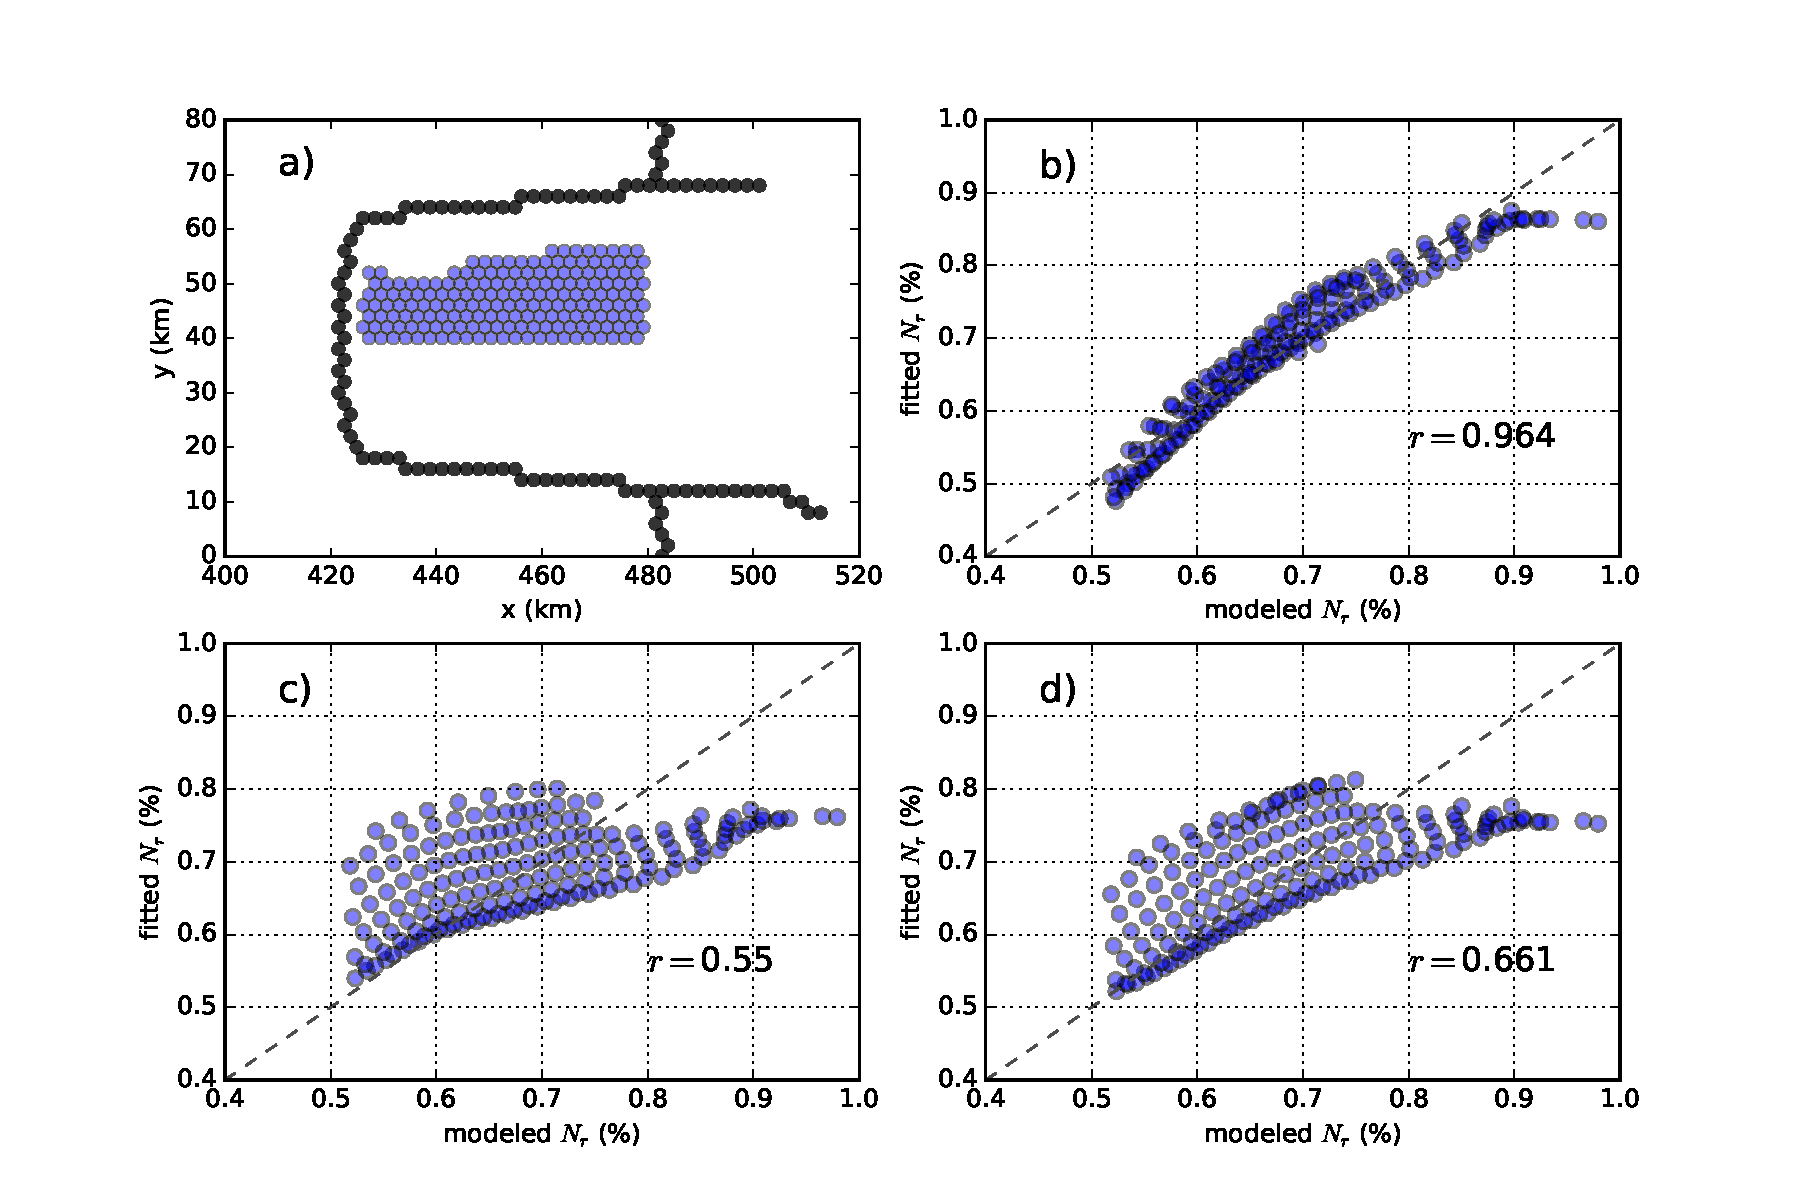
\includegraphics[width=1\linewidth]{figs/mismip_Nb_GLF_regression.pdf}
    \caption{(a) MISMIP+ steady-state geometry. Color represents the magnitude of the ice thickness gradient and the white line represents the GL. (b) $N_b$:$N_r$ correlation for all perturbation points. (c) $N_b$:$N_r$ correlation for perturbation points within the confined region of the shelf ($x>480$) and $>$10 km from the GL; (d) $N_b$:$N_r$ correlation for perturbation points within the confined region of the shelf and with a thickness gradient magnitude $\left|\nabla H\right|<7$x$10^{-3}$. In (c) and (d), the orange dots in the insets represent the GL grid cells, and the blue dots the perturbation grid cells. \textbf{SP: Matt suggested expanding this to include 2 more panels using the points in (d) -- the flow direction and the p2 direction (the goal being to show that the correlations are pretty bad). Then we could also add another panel along the bottom which is the 'continuous' version of these (i.e., the red curve in Fig. 3a).}}
\label{mismip_Nb_GLF_regression}
\end{figure}

%\subsection{The buttressing directions}
%\subsection{Correlation dependence on buttressing direction}
\subsection{Directional dependence of buttressing}

The buttressing number, $N_b$, is computed using the normal stress ($\sigma_{nn}$) projected onto a specific direction, see Equation (\ref{butN}). Therefore, the buttressing number at any perturbation point varies depending on the chosen direction. \citet{furst2016} calculated $N_b$ along two directions, the ice flow direction ($\mathbf{n}_f$) and the direction corresponding to the second principal stress ($\sigma_{p2}$) ($\mathbf{n}_{p2}$). They found that the latter---the direction corresponding to the maximum compressive stress (or the least extensional stress)---best identified ``passive'' regions, where the ice shelf provides little or no buttressing. In Fig.~\ref{mismip_r2_all_direction}, we plot the correlation coefficients ($r^2$) between $N_r$ and $N_b$ where the direction corresponding to $\sigma_{nn}$ varies continuously between 0 and 180$^\circ$ (as a function of the angle $\Delta \phi$) relative to the direction corresponding to the first principle stress ($\sigma_{p1}$) ($\mathbf{n}_{p1}$). We find the largest correlation coefficient ($r^2>0.9$) when $N_b$ is aligned with $\mathbf{n}_{p1}$ ($\Delta \phi=0^\circ$) and the smallest correlation coefficient ($r^2<0.4$) when $N_b$ is aligned with $\mathbf{n}_{p2}$ ($\Delta \phi=90^\circ$). We can also see the corresponding variations in buttressing number $N_b$ in Fig.~\ref{Nb_Deltaphi}, where the maximum buttressing number is calculated from $N_r(\mathbf{n}_{p2}$) according to Equation (\ref{butN}).
% for different directions with respect to the first principal stress and flow direction, respectively (Fig \ref{mismip_r2_all_direction}). Differently, we find that $N_b$ along the $\sigma_{p1}$ direction shows the best regression performance, whereas the $\sigma_{p2}$ appears to show the weakest correlations to $N_r$. This can be further testified by looking at the angle differences between $\sigma_{p1}$ and flow directions ($\Delta \phi = \phi_{flow}-\phi_{\sigma_{p1}}$). 

% As a second, somewhat independent check on the strong correlation between $N_r$ and $N_b$ as a function of the direction $\sigma_{p1}$, we also calculate the correlation coefficient for $N_b$ where the value for $\sigma_{nn}$ is calculated as a function of the ice flow direction. The blue line in Fig.~\ref{mismip_r2_all_direction}a is analogous to the red line but for the case where $\Delta \phi$ is relative to the ice flow direction. A similar sinusoidal pattern is evident, but with a phase lag of approximately $50^\circ$ relative to the red line. Thus, aligning the blue curve so that its maximum and minimum coincide with those of the red curve requires rotating the direction for calculating $\sigma_{nn}$ by $50^\circ$.    

A similar conclusion can be reached when the buttressing number is calculated by projecting $\sigma_{nn}$ onto $\mathbf{n}_{f}$\footnote{In \citet{furst2016}, the ice flow direction is the second direction considered when calculating the local ice shelf buttressing number (with the first direction considered being $\mathbf{n}_{p2}$).}. In Fig.~\ref{mismip_r2_all_direction}a, the blue line shows the $N_b$:$N_r$ correlation for the case of rotating relative to $\mathbf{n}_{f}$. %(the flow direction experiments are analyzed independently from the $\sigma_{p1}$ direction experiments, and can therefore be used as an approach for verification). 
For around 50\% of the perturbation points, the angles of flow directions are 30--50$^\circ$ ($\Delta\varphi$) more than that of the directions of first principle stresses (from Fig.~\ref{mismip_r2_all_direction}b), which is consistent with the phase difference between the blue and red curves in Fig.~\ref{mismip_r2_all_direction}a. For example, for the $\mathbf{n}_{f}$ curve (blue), we have the smallest value at $\Delta\phi\approx$ 38$^\circ$, i.e., 38$^\circ$ relative to the flow direction. Since the angles of $\mathbf{n}_{f}$ are 30--50$^\circ$ more than that of $\mathbf{n}_{p1}$, the lowest value should occur at 68--88$^\circ$ ($\Delta\phi+\Delta\varphi$) relative to $\mathbf{n}_{p1}$, which is corresponding to $\mathbf{n}_{p2}$. This is in consistent with the position of the smallest value for the $\sigma_{p1}$ direction curve (red; $\Delta\phi\approx$ 90$^\circ$). %\textbf{(SFP: See comments in source text regarding this paragraphy.)} 

%\textbf{TZ: I still feel we should keep the flow direction curve. Please see my responses in the source text.} 

Based on the discussion above and the work of \citet{furst2016}, it appears that $N_b(\mathbf{n}_{p2})$ provides a good indicator for the maximum buttressing at any location on the shelf and for identifying passive ice shelf areas. Yet it may not be a good metric for quantifying the sensitivity of GLF response to sub-shelf basal melt perturbations. In the following sections, we explain how and why changes in GLF are sensitive to the choice of direction when calculating the ice shelf buttressing number. 



\begin{figure}
\centering
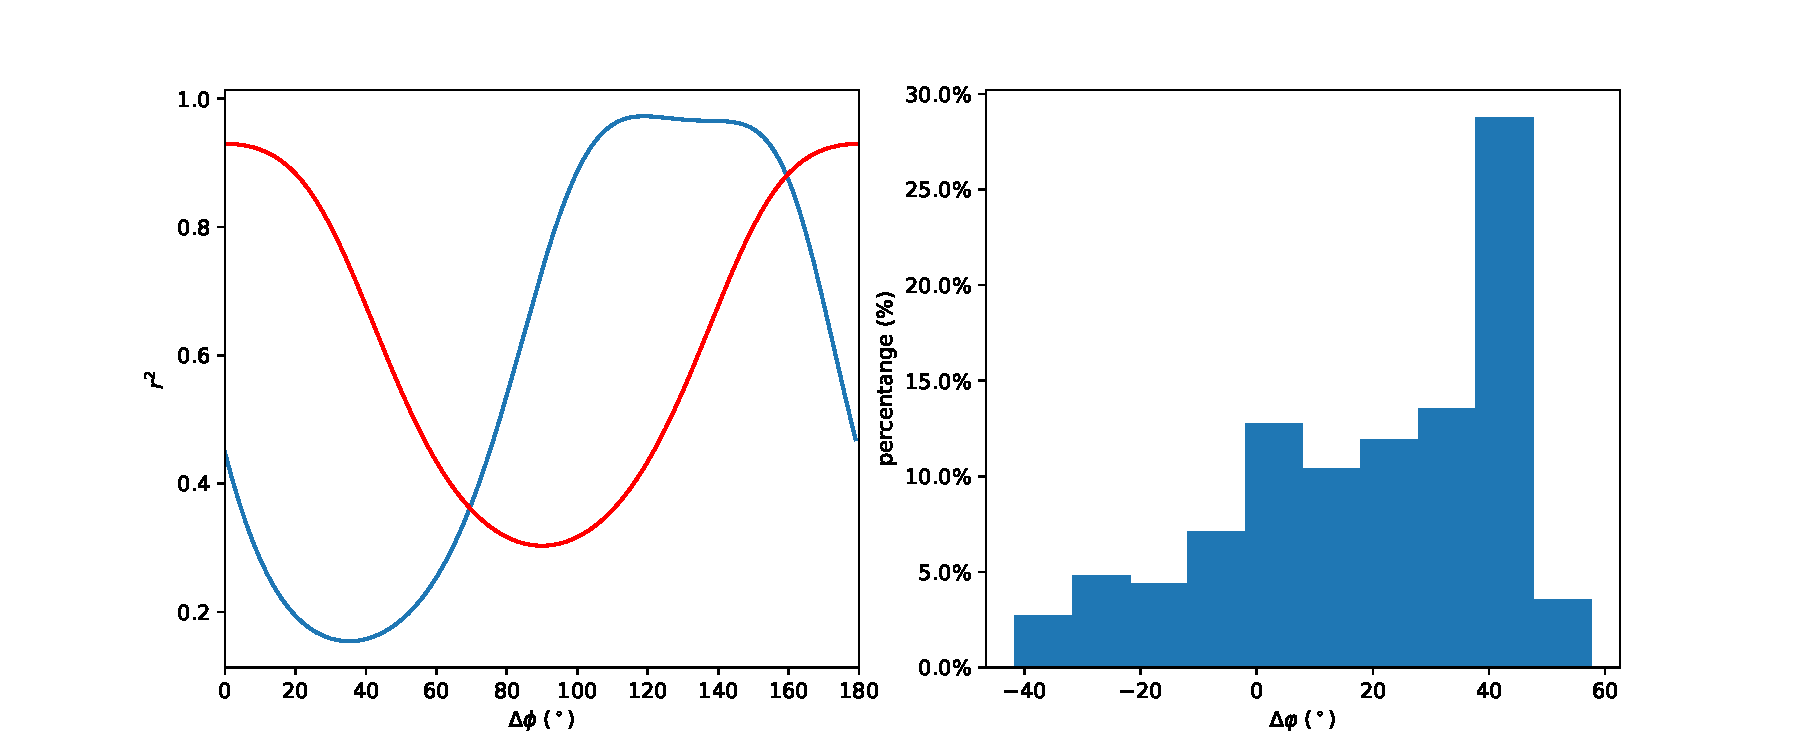
\includegraphics[width=1\linewidth]{figs/mismip_r2_all_direction.pdf}
    \caption{(a) $N_b$:$N_r$ correlation coefficients for $\sigma_{nn}$ values rotated counterclockwise by $\Delta\phi$ degrees relative to $\mathbf{n}_{p1}$ (red) and $\mathbf{n}_{f}$ (blue). (b) Histogram of the angular differences between $\mathbf{n}_{f}$ and $\mathbf{n}_{p1}$. The perturbation points analyzed here are those shown in the inset of Fig.~\ref{mismip_Nb_GLF_regression}d. \textbf{SP: Matt/Xylar suggested breaking the velocity part of this fig out into its own fig.}}
    \label{mismip_r2_all_direction}
\end{figure}

%\subsection{Possible controlling factors}
%\subsection{Understanding the dependence on buttressing direction}
%\subsection{Direction of velocity changes around perturbation points}
\subsection{Velocity changes in the vicinity of perturbation points}

The correlation between changes in GLF and normal stress (buttressing) directions can be partly understood by examining the spatial patterns of velocity change associated with thickness perturbations. %Further clues of the impacts from different chosen directions can be found in Fig.~\ref{perturb_theta_velchange}. 
In Fig.~\ref{perturb_theta_velchange}, we plot histograms of the maximum (red) and minimum (blue) speed changes around each perturbation point as a function of angular distance relative to $\mathbf{n}_{p1}$ ($\Delta\phi$, as in Fig.~\ref{mismip_r2_all_direction}a). That is, we count the number of neighboring cells that have maximum (most increased or least decreased) and minimum (most decreased or least increased) speed changes (for each cell, there is only one neighbor with maximum or minimum speed change).  %Figure \ref{perturb_theta_velchange} contains only the points from Fig.~\ref{mismip_Nb_GLF_regression}d (i.e., filtered according to ice thickness gradient). 
The maximum speed changes cluster within 0 to 45$^\circ$ of $\mathbf{n}_{p1}$ and the minimum speed changes cluster within 60 to 90$^\circ$, indicating that the majority of speed increases in the immediate region of a perturbation are more closely aligned with $\mathbf{n}_{p1}$ (and likewise, the majority of velocity decreases are more closely aligned with $\mathbf{n}_{p2}$). This finding supports the hypothesis that the thickness perturbations induce velocity increases along favored directions and that, for the MISMIP+ domain, $\mathbf{n}_{p1}$ is favored. 
\textbf{SP: I think it would help if we try to connect this more clearly to the next section. That is, here we show that a local perturbation leads to speed increases along preferred directions. Below, we show that local perturbations lead to similar speed increases (also along preferred directions) but at the GL.}

%\textit{... not sure how to close this yet. Something about how changes propagate more easily along p1 even though p2 ``controls'' the buttressing? Not sure we entirely understand this yet but we need to} \textbf{TZ: this section is an analysis of the velocity change (only) surrounded by the perturbation point. When there is a perturbation, its neighbor cells surrounded it will have different patterns of velocity change. In some directions the velocity increases and in other directions it decreases. Is there any patterns? For example, if the increase of velocity occurs along p1 or not?}.

\begin{figure}
	\centering
    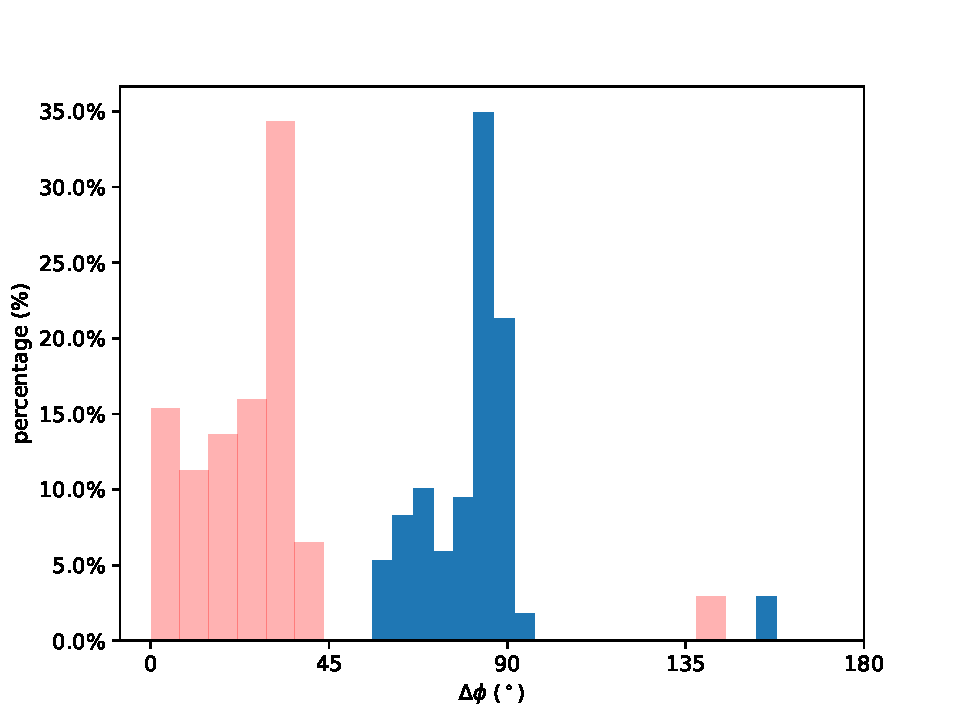
\includegraphics[width=1\linewidth]{figs/perturb_theta_velchange.pdf}
    \caption{Histograms for the maximum (red) and minimum (blue) percent speed change in grid cells adjacent to a thickness perturbation point, plotted as a function of angular distance with respect to the $\sigma_{p1}$ direction. Points analyzed are those from Fig.~\ref{mismip_Nb_GLF_regression}d.}
	\label{perturb_theta_velchange}
\end{figure}

%\subsection{The changes of velocity and stress along GL}
\subsection{Speed and stress changes along the GL}

Further insight into the importance of $\mathbf{n}_{p1}$ is given by examining changes in the state of stress and velocity as a result of a perturbation in local ice thickness. To this end, we define the metric $\Upsilon$,  
\begin{equation}
    \Upsilon= \textrm{Corr}\left(\frac{\sigma_{p}-\sigma_{c}}{\sigma_{c}}, \frac{u_{p}-u_{c}}{u_{c}}\right),
\label{upsilon}
\end{equation}
%\begin{equation}
%    \Psi= \frac{\sigma_{p}-\sigma_{c}}{\sigma_{c}}-\frac{u_{p}-u_{c}}{u_{c}},
%\label{psi}
%\end{equation}
\textbf{SP: need to update this equation to clarify the following things: 1) upsilon is scalar function of x,y (that is, we calculate a single value of it for each perturbation point on the ice shelf), 2) the two terms in parentheses are vectors of points along the GL, 3) the operation here is a dot product, so that the vectors collapse to a scaler value, which is what is evalutated).}
where the subscripts $p$ and $c$ denote the perturbation experiments and the ``control'' (i.e., the initial condition), respectively, and $\sigma$ and $u$ denote the stress component and ice speed along the GL, respectively. $\Upsilon$, a correlation coefficient, is a measure of the consistency between the magnitude and sign of the change in the model stress and velocity states along the GL between the control and perturbation experiments. We calculate $\Upsilon$ for every perturbation point and for all directions in the span of $\Delta\phi=$0--180$^\circ$ relative to $\mathbf{n}_{p1}$ (Fig.~\ref{stress_vel_corr_GL_allP}). For normal stress perturbations relatively more parallel to $\mathbf{n}_{p1}$ (closer to 0$^\circ$ or 180$^\circ$), there is a much stronger correlation between changes in normal stress and changes in ice surface speed (and hence the ice flux) than for normal stress perturbations that are relatively more parallel to $\mathbf{n}_{p2}$ (closer to 90$^\circ$).  
\begin{figure}
	\centering
    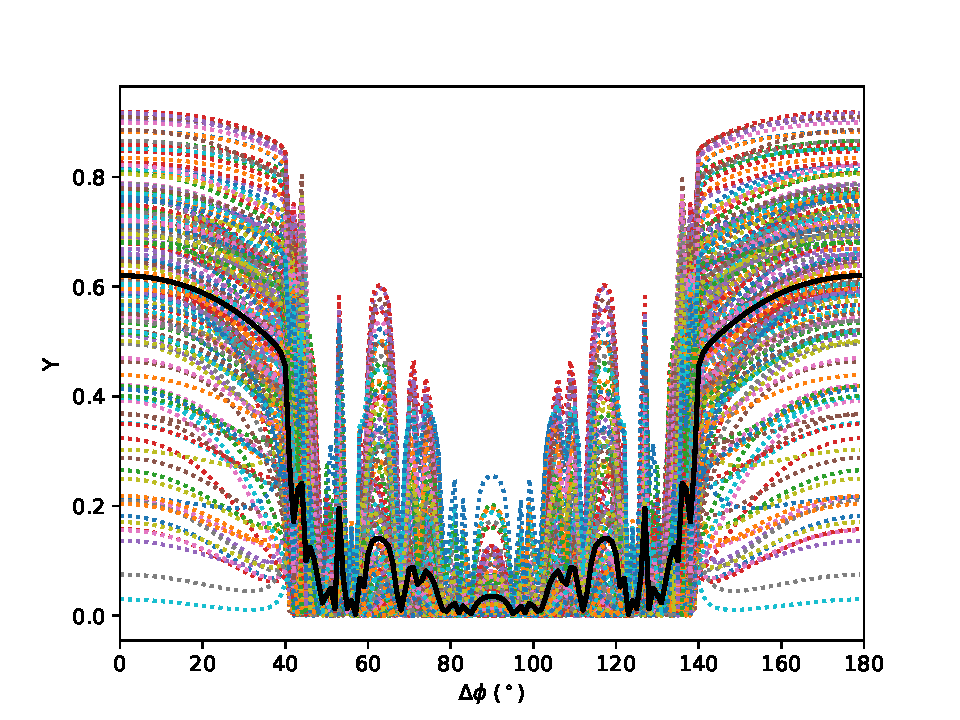
\includegraphics[width=1\linewidth]{figs/stress_vel_corr_GL_allP.pdf}
    \caption{Correlation between the change in normal stress and the change in ice surface speed along the GL (i.e., $\Upsilon$ from (\ref{upsilon})). The horizontal axis shows how $\Upsilon$ varies as a function of the direction of the normal stress, rotated counterclockwise from $\mathbf{n}_{p1}$. Colored, dotted curves each represent a single perturbation experiment and the thick black curve is their mean for a given value of $\Delta\phi$. \textbf{SP: We should swap the order of this figure with the next one, since this is the 'continuous' version of that one (see related note in caption below).}}
	\label{stress_vel_corr_GL_allP}
\end{figure}
By plotting spatial maps of $\Upsilon$ for every perturbation point of interest in the domain, we show that there is generally a stronger correlation, in general, between changes in normal stress and velocity along $\mathbf{n}_{p1}$ (Fig.~\ref{stressDiff_velDiff_GL_allPerturb}a) than along $\mathbf{n}_{p2}$ (Fig.~\ref{stressDiff_velDiff_GL_allPerturb}b).  
%for the case where $\sigma_{nn}$ in (\ref{butN}) is set equal to $\sigma_{p1}$ (Fig \ref{stressDiff_velDiff_GL_allPerturb}a) and $\sigma_{p2}$ (Fig \ref{stressDiff_velDiff_GL_allPerturb}b). From Fig.~\ref{stressDiff_velDiff_GL_allPerturb}, it is clear that the correlation between stress and velocity change along GL is generally much larger in the MISMIP+ domain for the case of $\sigma_{nn}=\sigma_{p1}$, especially for some regions in the center of the domain. \textit{SP: Or something like this. Need to think about it some more still. I wonder if it could also be interpreted differently---e.g., in 5b, could the much larger variance be because a small change in p2 results in a much larger change in velocity (relative to p1)?. Would it make more sense for Fig. 5 to be an actual correlation coeff. plot rather than the somewhat complicated variance comparison?}. \textbf{TZ: I now change deviation to correlation. You are right. It's more consistent. I think the problem is to check if the changes of $\sigma_{p1}$ or $\sigma_{p2}$ can cause more consistent velocity changes along GL, right? For example, if $\sigma_{p2}$ can cause a larger but more consistent change in vel. than $\sigma_{p1}$, then $\sigma_{p2}$ is still the better metric than $\sigma_{p1}$.} 
%In Fig.~\ref{vel_stress_change_example} we show the stress and velocity changes at the GL for a perturbation at a specific location on the ice shelf, which may provide a more clear evidence of a strong (weak) correlation between changes in the first principal stress (second principal stress) and changes in the velocity (Fig.~\ref{vel_stress_change_example}). For this particular perturbation spot, we can also see the changes of buttressing number calculated by $\sigma_{p1}$ (Fig.~\ref{sigma_change_example}a) and $\sigma_{p2}$ (Fig.~\ref{sigma_change_example}b) across the domain. In this case the buttressing number calculated from $\sigma_{p1}$ shows more decrease than that from $\sigma_{p2}$ for most upstream parts to the perturbation spot, indicating another evidence that the more tensile stress $\sigma_{p1}$ can change more significantly and therefore contribute more to the changes of ice shelf buttressing under certain basal melt forcing scenarios. 
If we plot the change in $N_b$ between the perturbation and control experiments at every point for $N_b(\mathbf{n}_{p1})$ (Fig.~\ref{sigma_change_example}a) and for $N_b(\mathbf{n}_{p2})$ (Fig.~\ref{sigma_change_example}b), we see that the reduction in buttressing is generally larger in magnitude, more spatially extensive, and more aligned with the mean ice flow direction (left to right in Fig.~\ref{sigma_change_example}) for the case of $N_b(\mathbf{n}_{p1})$ (Fig.~\ref{vel_stress_change_example} shows a detailed comparison between the change in stress and velocity along the GL for a single perturbation on the ice shelf). 

%We can also see the changes of buttressing number calculated by $\sigma_{p1}$ (Fig.~\ref{sigma_change_example}a) and $\sigma_{p2}$ (Fig.~\ref{sigma_change_example}b) across the domain. In this case the buttressing number calculated from $\sigma_{p1}$ shows more decrease than that from $\sigma_{p2}$ for most upstream parts to the perturbation spot, indicating another evidence that the more tensile stress $\sigma_{p1}$ can change more significantly and therefore contribute more to the changes of ice shelf buttressing under certain basal melt forcing scenarios. 

% This possibly indicates that GLF are more relevant to the changes of $\sigma_{p1}$ along GL, compared to the $\sigma_{p2}$ case, which can be clearly found if we look at some specific perturbation example as shown in Fig.~\ref{vel_stress_change_example}. 

\begin{figure}
	\centering
    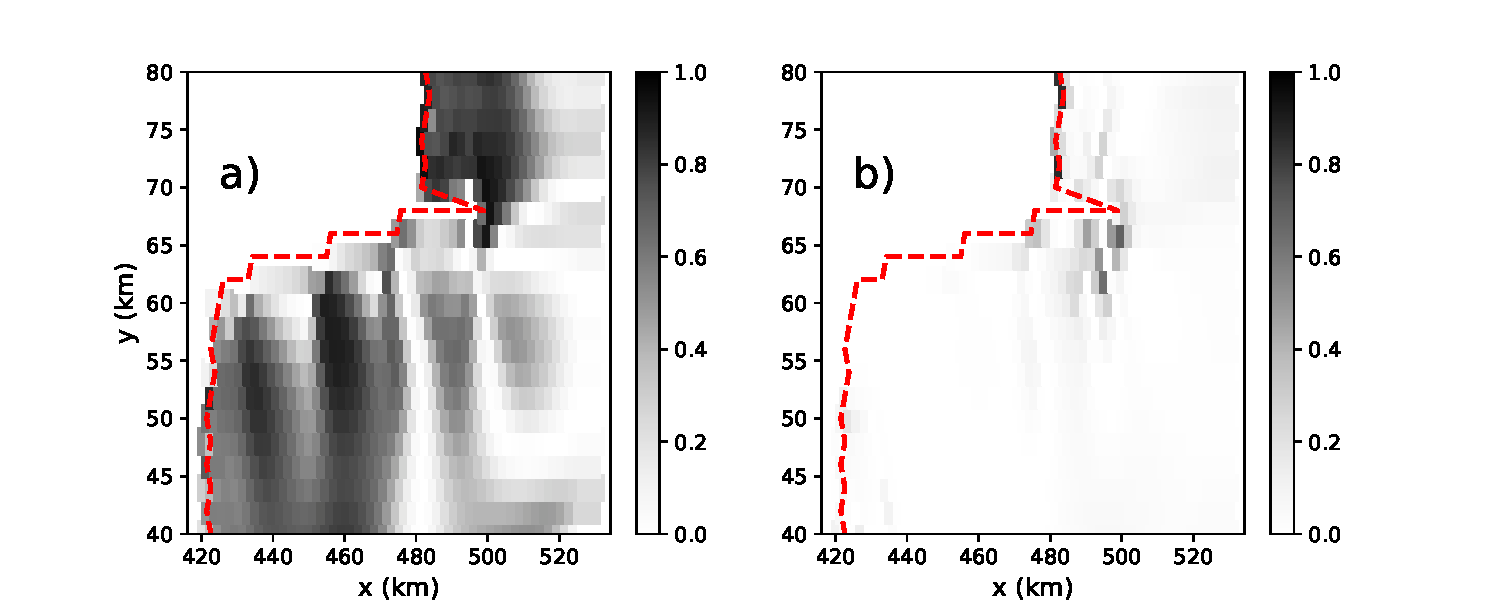
\includegraphics[width=1\linewidth]{figs/stressDiff_velDiff_GL_allPerturb.pdf}
    \caption{Spatial maps of the correlation coefficient $\Upsilon$ from Equation (\ref{upsilon}) over the MISMIP+ domain for normal stress changes calculated parallel to (a) $\mathbf{n}_{p1}$  and (b) $\sigma_{p2}$. Note that $\Upsilon$ is a metric for the changes of stress and speed along GL. \textbf{SP: Swap the order of this fig w/ the one above, since this shows what Upsilon looks like along only two directions (while that figure shows the 'continuos' form of Upsilon).}}
	\label{stressDiff_velDiff_GL_allPerturb}
\end{figure}

%\textit{SP: Leaving this section alone for now. I think it's worth including some additional discussion here if we can make some reasonable speculation as to what's going on \textbf{TZ: The metric regarding distance and flow/stress angle is a such speculation that the impact of perturbation on GLF is a combined effect of perturbation and GL dynamics (see below)}. But we probably need to come up with a bit more than this. I wonder if there are other T3 folks who might have some insight into this problem \textbf{TZ: there might be some similar theory going on here, but I doubt the pure mechanical knowledge apply in this specific problem. Perhaps Xylar can contribute a bit from the perspective of Fourier transform theory} ? One thing that occurs to me is that we could be conflating cause and effect here. For example, when we look at Figure 6, it looks like the changes in velocity correlate with changes in $\sigma_{p1}$, whereas they don't correlate with changes in $\sigma_{p2}$. But it could simply be that the changes in $\sigma_{p2}$ (due to the thickness perturbation) are causing a velocity change, and the velocity change is better reflected by the change in $\sigma_{p1}$. This makes sense at the GL, where we know the velocity / flux are largely going to be aligned with the $\sigma_{p1}$ direction (perpendicular to the GL). This doesn't, however, explain why we see a good correlation between changes in velocity / flux at the GL (reflected by the flux response number, N) and $\sigma_{p1}$ but a much poorer correlation between the flux response number and $\sigma_{p2}$. \textbf{TZ: I am not sure if I follow you here. I don't know if it's a proper way to say that the changes in $\sigma_{p2}$ cause the changes in velocity. If we look closely at Fig.~\ref{vel_stress_change_example} we can see that for some cells on GL, even though the velocity direction is more aligned with p1, the correlation is still poor, whereas the correlation with p2 is better for these same cells. The difference here is their respective angle difference with the stress direction at perturbation spot (a main reason I make up the metric in the following; I can show you some point when you have time). It's hard to know exactly the reason behind.}} 

One possible reason that we might see such direction-dependent correlations might be due to the way perturbations propagate through ice shelves. The energy of from a perturbation propagates with the group velocity, which can be analyzed using a Fourier transform, similarly to \citet{gudmundsson2003}. Using simplified geometry, \citet{gudmundsson2003} analyzed the propagation of basal perturbation to glacier surface and found that the direction of group velocity is aligned closely with the main flow. The existence of a preferred propagation direction for the perturbations can possibly lead to our findings that favor the first principal stresse directions. 
%(\textbf{TZ: I am still not able to explain why it's exactly the first principal stress direction :(   SP: Let's leave this for now and see if we get some more useful input from co-authors. But, we do need to close this section somehow and it makes sense to do that by speculating a bit more on why we think this correlation between GLF changes and the p1 direction exists.} \textbf{TZ: from what I understand such preferred direction appears based on the fact that the ice dynamics at GL is preferably controlled by some normal stress along certain direction, say, $\sigma_{p1}$.}
\textbf{SP: At the end of this section, it would be useful to summarize what these two sections (and figs 4, 5, 6) tell us. That is, that one possible explanation for the strong correlation between GLF changes and buttressing calculated in the p1 direction is that local perturbations in thickness trigger velocity increases along favored directions. And, for both local and distal (at the GL) increases in velocity, those favored directions are also aligned with the p1 direction. We might think about more clearly joining these two sections into a single chunk of discussion by putting the 'velocity changes in the vicinity of ...' and 'speed and stress changes ...' sections above under a single broader section, called something like 'Directional dependence of changes in velocity' (which then jibes a bit better with the title of the section above).}

% \begin{figure}
% 	\centering
%     \includegraphics[width=1\linewidth]{figs/vel_stress_change_example_new.pdf}
%     \caption{Relationship between GL {changes} in the velocity (blue) and in the stress (red) for the MISMIP+ test case due to a perturbation at a specific location on the ice shelf (blue dot in inset map). In a), changes in GL velocity are plotted against changes in $\sigma_{p1}$ and in b) changes in GL velocity are plotted against changes in $\sigma_{p2}$. The $x$-axis is an index for the grid cell number along the GL.}
% 	\label{vel_stress_change_example}
% \end{figure}

\begin{figure}
	\centering
    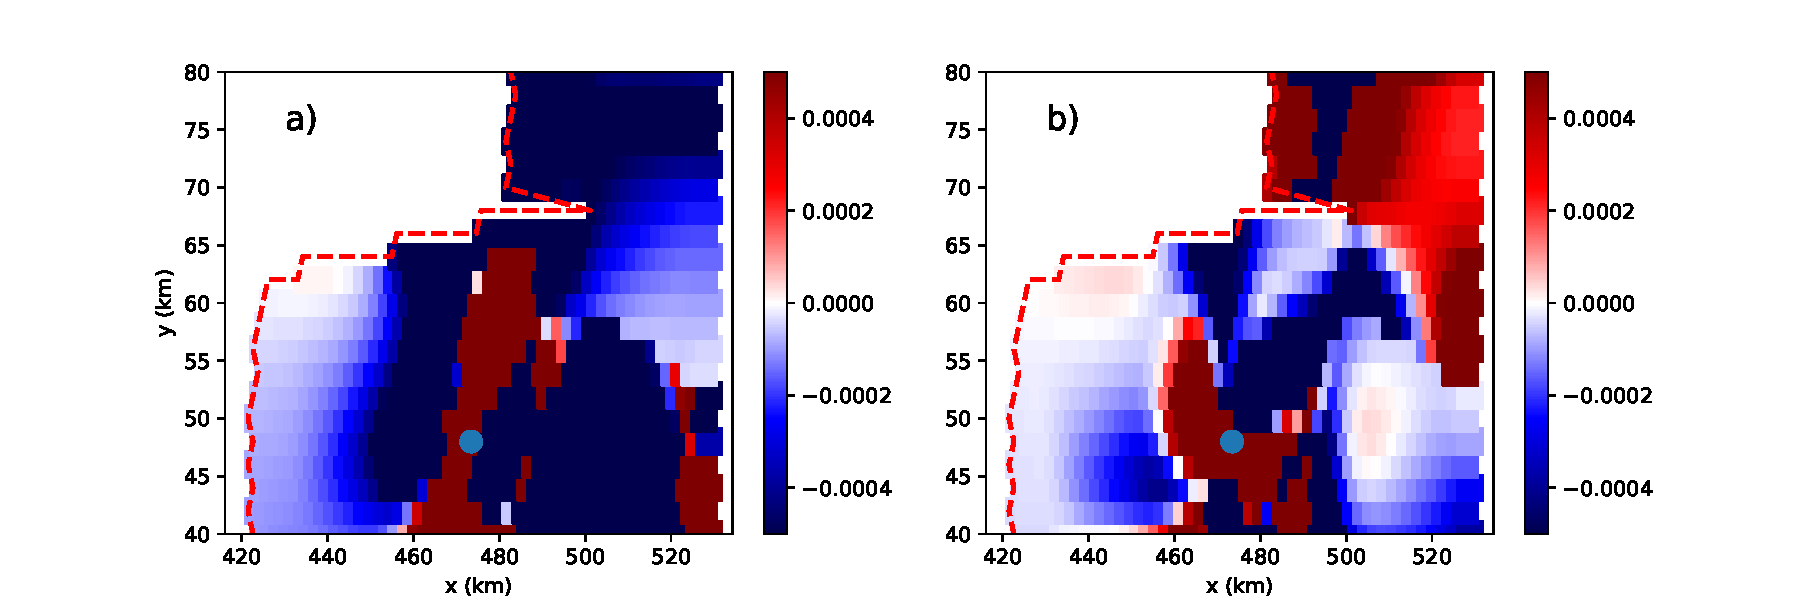
\includegraphics[width=1\linewidth]{figs/sigma_change_example.pdf}
    \caption{The percentage changes of buttressing number across the MISMIP+ (half) domain under the perturbation shown as the blue circle. In a) and b), the buttressing numbers are calculated along $\mathbf{n}_{p1}$ and $\mathbf{n}_{p2}$, respectively.}
	\label{sigma_change_example}
\end{figure}

\subsection{A metric connecting perturbations in thickness to changes in GLF}
\textbf{SP: I think we might want to copy/paste this whole section into the appendix for the time being. In some of the discussion with Xylar and Matt, we decided this does not necessarily add any new information that we don't already know from other calculations above (e.g., it uses/needs a lot of the same information that we currently show in fig 3 above) but it is much harder to understand. At this point, I think we know we aren't going to find a better simple metric than just the buttressing number using the p1 direction, so it doesn't make sense to try to introduce a more complicated one (and we're going to advocate for the adjoint approach in the end anyway).}
The change in GLF for a given perturbation to the ice-shelf thickness must be controlled by both the perturbation itself (the local change to the geometry, stress, and velocity fields) and the broader, surrounding ice dynamical setting (the regional geometry, stress, and velocity fields). To explore this further, we propose the following simplified metric, which connects and combines local aspects of a perturbation with its regional impact on GLF:
\begin{equation}
    \Lambda = \sum_i^I \frac{1}{d_i} |\mathrm{cos} \left(\theta_i\right)|,
    \label{Lambda}
\end{equation}
where $I$ is the total number of grid cells along the GL, $d_i$ is the distance between the perturbation point and the $i$-th GL grid cell, and $\theta_i$ is the angular difference between the direction of the specified normal stress (e.g., $\sigma_{p1}$) at the perturbation point and the flow direction for the $i$-th GL grid cell. The metric $\Lambda$ thus aims to capture two important factors impacting changes in GLF as a function of perturbations in ice shelf thickness: 1) the distance between the perturbation point and the GL (intuitively, the closer the perturbation to the GL, the larger the impact---also see the related discussion in the next section). We note that, while this metric does not \textit{explicitly} account for kinematic or dynamical processes (i.e., there are no terms explicitly involving velocities or stresses), it accounts for them \textit{implicitly} through the term in the numerator, which requires knowledge of the velocity and stress directions. 

Similar to above, we rotate the buttressing direction by 0--180$^\circ$ with respect to $\mathbf{n}_{p1}$, and calculate $\Lambda$ for each perturbation point. From Fig.~\ref{new_metric_new} we can see that $\Lambda$ has large values when the buttressing directions are close to $\mathbf{n}_{p1}$ ($\Delta\phi=0^\circ$ or $\Delta\phi=180^\circ$). A possible reason is that, for the MISMIP+ geometry, the velocity across the GL (and thus the GLF) is largely parallel with the $\sigma_{p1}$ direction at the GL (see Fig.~\ref{principal_stress_quiver}). This, in turn, is largely the result of extensional flow across the majority of the MISMIP+ GL.
%For grid cells where $\sigma_{p2}$ is also important, we can also see good matches between the changes of velocity and $\sigma_{p2}$ on GL, for example, grid cell number 65--75 and 90--95 in Fig.~\ref{vel_stress_change_example}b. 
For real ice shelves, where the pattern of ice flow across the GL is generally more complex (e.g., in the presence of an ice rise downstream from the GL), we expect a metric based on the assumption that $\sigma_{p1}$ and changes in GLF are well correlated to be less robust
.  


\begin{figure}
	\centering
    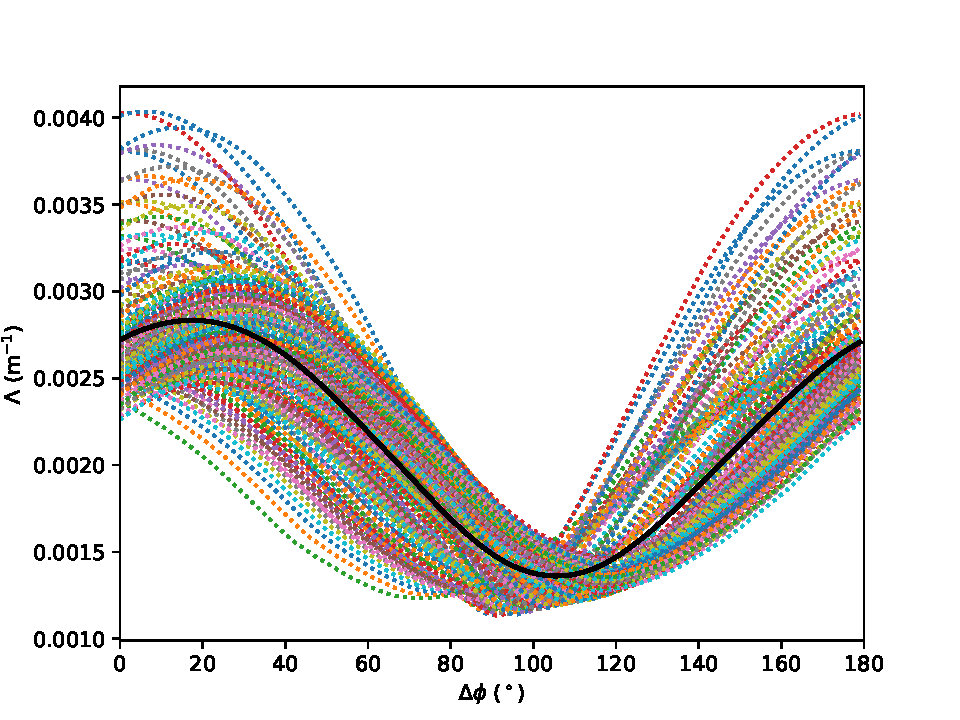
\includegraphics[width=1\linewidth]{figs/new_metric_new.pdf}
    \caption{A metric that gives a possible explanation of the connection between perturbation and GLF. Same as above, $\Delta\phi$ is the angular distance from the direction of $\sigma_{p1}$. The line types are the same as in Fig.~\ref{stress_vel_corr_GL_allP}}
	\label{new_metric_new}
\end{figure}


\subsection{Application to Larsen C Ice Shelf}

To explore whether the $N_b$:$N_r$ correlations found for the MISMIP+ test case hold for realistic ice shelves, we apply a similar analysis to our Larsen C domain. In this case, the computational mesh resolution varies, from finer near the GL (2 km) to coarser towards the center of the ice shelf and calving front (6 km). In order to be comparable to the experiments and results of \citet{reese2018}, we use 20 km $\times$ 20 km boxes for the application of ice-thickness perturbations, where the number of grid cells contained within each perturbation ``box'' is adjusted to sum to their correct total area. Additionally, to investigate the impacts of the complex geometry of the Larsen C Ice Shelf (i.e., the GL shape, the existence of ice rises, etc.), we apply two sets of perturbation experiments for which the 20 km $\times$ 20 km averaging boxes both do and do not include perturbations applied to cells near the GL. % for investigating further the nonlinearity feature we observe in the above MISMIP+ section. 

Analogous to Figures \ref{mismip_r2_all_direction}a,b for the MISMIP+ test case, Figures \ref{larsenc_r2_all_direction}a,b shows the $N_b$:$N_r$ correlations for the Larsen C model domain (including only perturbation points that are $>$50 km away from both the calving front and the GL). As previously, calculating $N_b$ using $\sigma_{nn}$=$\sigma_{p1}$ provides the best overall correlation between $N_b$ and $N_r$ (red curve for $\Delta\phi=0^\circ$) and calculating $N_b$ using $\sigma_{nn}$=$\sigma_{p2}$ provides the worst overall correlation (red curve for $\Delta\phi=90^\circ$). The phase difference between the $\sigma_{p1}$ and flow direction results can also be partially explained by their respective angle differences. In Fig.~\ref{larsenc_r2_all_direction}b we can find the local flow direction is typically oriented around 90--100 degrees counterclockwise of the local $\sigma_{p1}$ direction. This is a bit biased than the around 70 degree difference in Fig.~\ref{larsenc_r2_all_direction}a. However, considering the stress values (and thus $N_b$) for each perturbation box are averaged over multiple cells, we argue this difference is probably an acceptable error during our calculation. \textbf{SP: As noted above, I'm not sure about introducing the discussion about results relative to the velocity direction, as I think they are maybe just confusing. So leaving this part of the text alone for now.} \textit{\textbf{TZ: Personally I prefer to let the flow direction curve remain. I think this may give the reader more confidence of our results. I'll also wait Matt and Xylar's opinions about this.}} 

In Figures \ref{larsenc_r2_all_direction}c,d we redo the same analysis but include points near the GL (more than 10 km away from the calving front with a thickness gradient $\left|\nabla H\right|< 2 \times$10$^{-3}$). This reduces the $r^2$ values by a factor of two and also changes the relationship between the correlation coefficient and the alignment relative to $\sigma_{p1}$. Specifically, while the direction aligned with $\sigma_{p2}$ still gives the worst $N_b$:$N_r$ correlation, the direction giving the best correlation is rotated by approximately $40^\circ$ relative the direction associated with $\sigma_{p1}$. This indicates that thickness perturbations at these locations are propagating, at least in part, along both the $\sigma_{p1}$ and $\sigma_{p2}$ directions and leading to increases in GLF. In addition, there is no clear relationships between changes of velocity and specified normal stresses along the GL for Larsen C Ice Shelf (Fig.  \ref{stress_vel_corr_GL_allP_larsenC}), as their is for the MISMIP+ domain (\ref{mismip_r2_all_direction}), due to the complex geometry and ice flow along the GL \textbf{TZ: A thought: I am not sure if it can get better if we pick some of the cells with simpler geometry on GL.}. \textit{SP: I'm not really sure what else we can say about this, other than that it's an indication that using $\sigma_{p1}$ and $\sigma_{p2}$ in the calculation of $N_b$ is probably just more problematic for complex geometries. I think it's fair to leave it at that in this paragraph, since overall, we know that the main conclusions are going to be that this type of analysis appears to be of limited use on realistic geometries for a few different reasons.} 
%Although the angle differences between the flow and $\sigma_{p1}$ directions are still mostly near 90 degree, there are no longer clear patterns in the phase differences for the corresponding $r^2$ curves. In addition, the $\sigma_{p1}$ directions are also no longer indicating the best $r^2$ correlations. However, the directions along $\sigma_{p2}$ appears to still pointing to the weakest $N_b$-$N_r$ correlations, despite the overall much smaller $r^2$ values in this case.


\begin{figure}
	\centering
    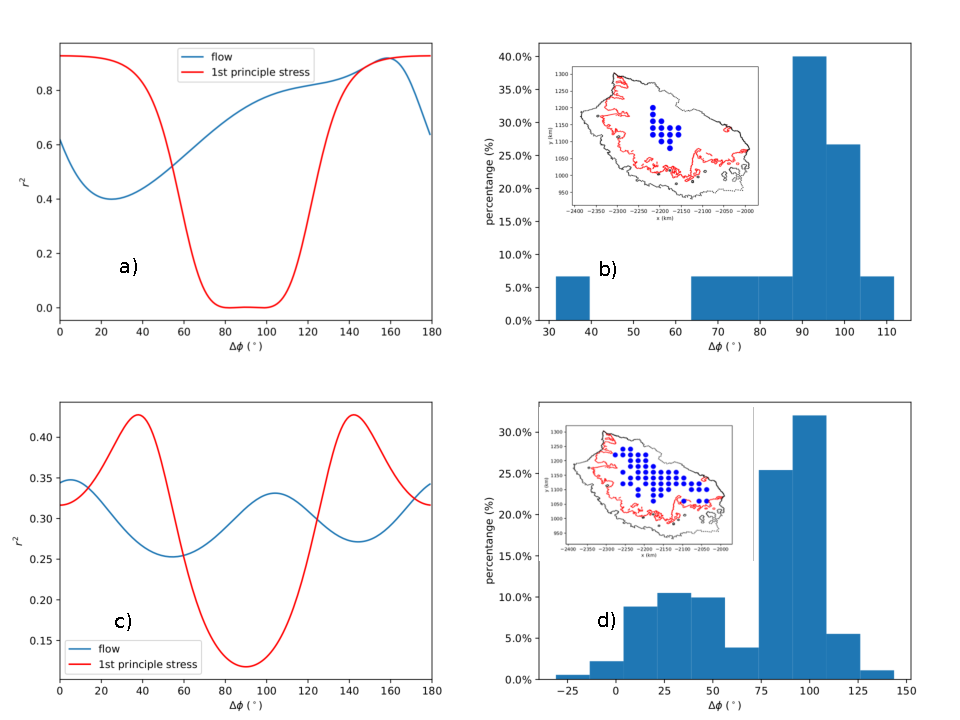
\includegraphics[width=1\linewidth]{figs/larsenc_r2_all_direction.pdf}
    \caption{(a, c) The $N_b$:$N_r$ correlation coefficients for each direction rotated counterclockwise from the $\sigma_{p1}$ (red) and flow direction (blue). (b, d) The histogram of the angular differences between the ice flow and $\sigma_{p1}$ directions. The insets in b) and d) show the locations of the 20 km $\times$ 20 km perturbation boxes (blue circles). \textbf{SP: We could make this plot simpler/smaller by removing the vel correlations and histograms and just including the red lines and the maps. Especially if we don't think the flow direction based metric is useful and we don't spend anytime talking about it.}}
	\label{larsenc_r2_all_direction}
\end{figure}

%\subsection{Impacts of near-GL perturbations}
\subsection{The impact of perturbations applied near the GL}

For thickness perturbations applied near the Larsen C GL, the correlations between buttressing number and changes in GLF discussed above (e.g., Figs.~\ref{mismip_Nb_GLF_regression}, \ref{mismip_r2_all_direction}) do not obviously hold. This may be due to an additional dependence on the distance between the GL and perturbation locations or on particular, nearby geometric features. While a perturbation decays over distance \citep{lick1970}, cells at the GL  that are near to a perturbation location will be impacted by that perturbation relatively easily. This can be verified by looking at the standard deviations of GL velocity change due to each perturbation (Fig.~\ref{vel_change_std}). For a perturbation applied close to the GL, the corresponding GLF change is, in general, confined to a local region near that perturbation. On the other hand, the impact on the GLF in areas far from that local region are small (resulting in large standard deviations; also see Fig.~\ref{mismip_larsenc_dist}). A practical implication of this finding is that strong spatial heterogeneity in GL retreat could result from ice shelf thickness perturbations (e.g., submarine melting) applied very close to the GL. 

The propagation of perturbations is also strongly impacted by the geometry of the GL. For example, in the MISMIP+ test case the perturbations near $480 < x < 500$\,km and $y = 65$\,km in Fig.~\ref{vel_change_std}a cannot impact the ice flow on the other side of the grounded peninsula, at 480 $<$ x $<$ 500 km and 70 $<$ y $<$ 80 km (see also Fig.~\ref{mismip_larsenC_velChange}a). For a perturbation within a local embayment of the Larsen C Ice Shelf, the embayment itself ``shades'' the majority of the rest of the Larsen C GL from the impacts of the perturbation (Fig.~\ref{mismip_larsenC_velChange}b). This is one of the primary factors complicating the use of the buttressing number as a practical metric for diagnosing GLF sensitivity on  real ice shelves.
 
\begin{figure}
	\centering
    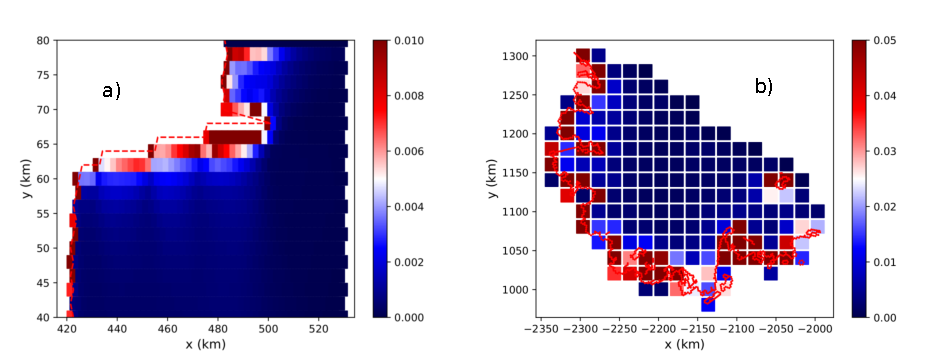
\includegraphics[width=1\linewidth]{figs/vel_change_std.pdf}
    \caption{Standard deviation of velocity change along GL for each perturbation point for the MISMIP+ (a) and Larsen C (b) experiment. The red dashed lines (points) are the GLs for MISMIP+ (a) and Larsen C (b) .}
	\label{vel_change_std}
\end{figure}

\subsection{Adjoint sensitivity}

Motivated by some of the complications discussed above when looking for a simple metric for diagnosing GLF sensitivity to local ice shelf thickness changes, we now investigate a different approach. This approach provides a sensitivity map of the GLF analogous to the one proposed and discussed above but associated to infinitesimal rather than finite perturbations. Instead of computing the GLF change due to individual perturbations at each \textit{n} model grid cells, requiring \textit{n} forward solves, the adjoint method allows to compute the sensitivity at all  cells simultaneously at the cost of a single linear solve. Briefly, this method involves the solution of an auxiliary linear system (the adjoint system) to compute the so-called Lagrange multiplier (a variable that has the same dimension of the velocity solution). The matrix associated to the system is the transpose of the Jacobian of the first-order flow model. In addition, the adjoint method requires the computation of the partial derivatives of the FO residual and the GLF w.r.t. the velocity solution and the ice thickness. We compute the Jacobian and all the other derivatives using automatic differentiation.
We note that the computation of the derivatives require special attention because a change in the thickness affects the geometry of the problem, and so shape derivatives need to be taken into account as well.
A similar adjoint approach has been proposed in \cite{Goldberg2019} to compute the sensitivity of the volume above flotation w.r.t the melting rate averaged over the period 2011-2015. In contrast to our approach, the authors have to compute \emph{transient} sensitivities because their quantity of interest is averaged over a period of time.  

%Once the Lagrangian multiplier has been computed, the sensitivity map can be computed by evaluating the derivative w.r.t. the with a matrix vector multiplication, where the  is given by the contraction of the Lagrange multiplier with the 
%This approach provides results analogous to those presented and discussed above but at a greatly reduced cost: rather than using the forward model to examine the sensitivity of GLF change to individual perturbations at each of \textit{n} model grid cells, we use a single adjoint solve to deduce those same sensitivities at all \textit{n} grid cells \textit{simultaneously} from the tangent linear model. 

%Briefly, this method involves ... 
%\textit{Mauro, please give us a sketch of some technical details here and we can fill in the rest.}

In Fig.~\ref{adjoint_comp}, we provide a demonstration of this method for the case of the MISMIP+ domain by comparing sensitivities deduced from 730 individual forward model evaluations (i.e., the perturbation experiments discussed above, which are analagous to those in \citet{reese2018}) with those deduced from a single model adjoint solve. Here, the ``sensitivity'' is defined as ... \textit{SP: need more details from Mauro here.} 

The comparison in Fig.~\ref{adjoint_comp} demonstrates that, for points in the domain we expect to be comparable, the two approaches provide a near exact match. The two methods disagree in regions very near to the GL (see Fig.~\ref{adjoint_comp_appendix}), which we hypothesize to be the result of nonlinearities near the GL that prevent accurate use of the tangent linear model for deducing sensitivities. This method provides clear advantages over the more \textit{ad hoc} analysis methods discussed above in that, in addition to providing a map of where the GLF is most sensitive to local ice thickness changes, the impact of those thickness changes on GLF flux can be calculated directly from the value of the sensitivity. \textit{SP: I wonder if we also want to show a map of those sensitivities (with units) in the appendix somewhere.}  

\begin{figure}
	\centering
    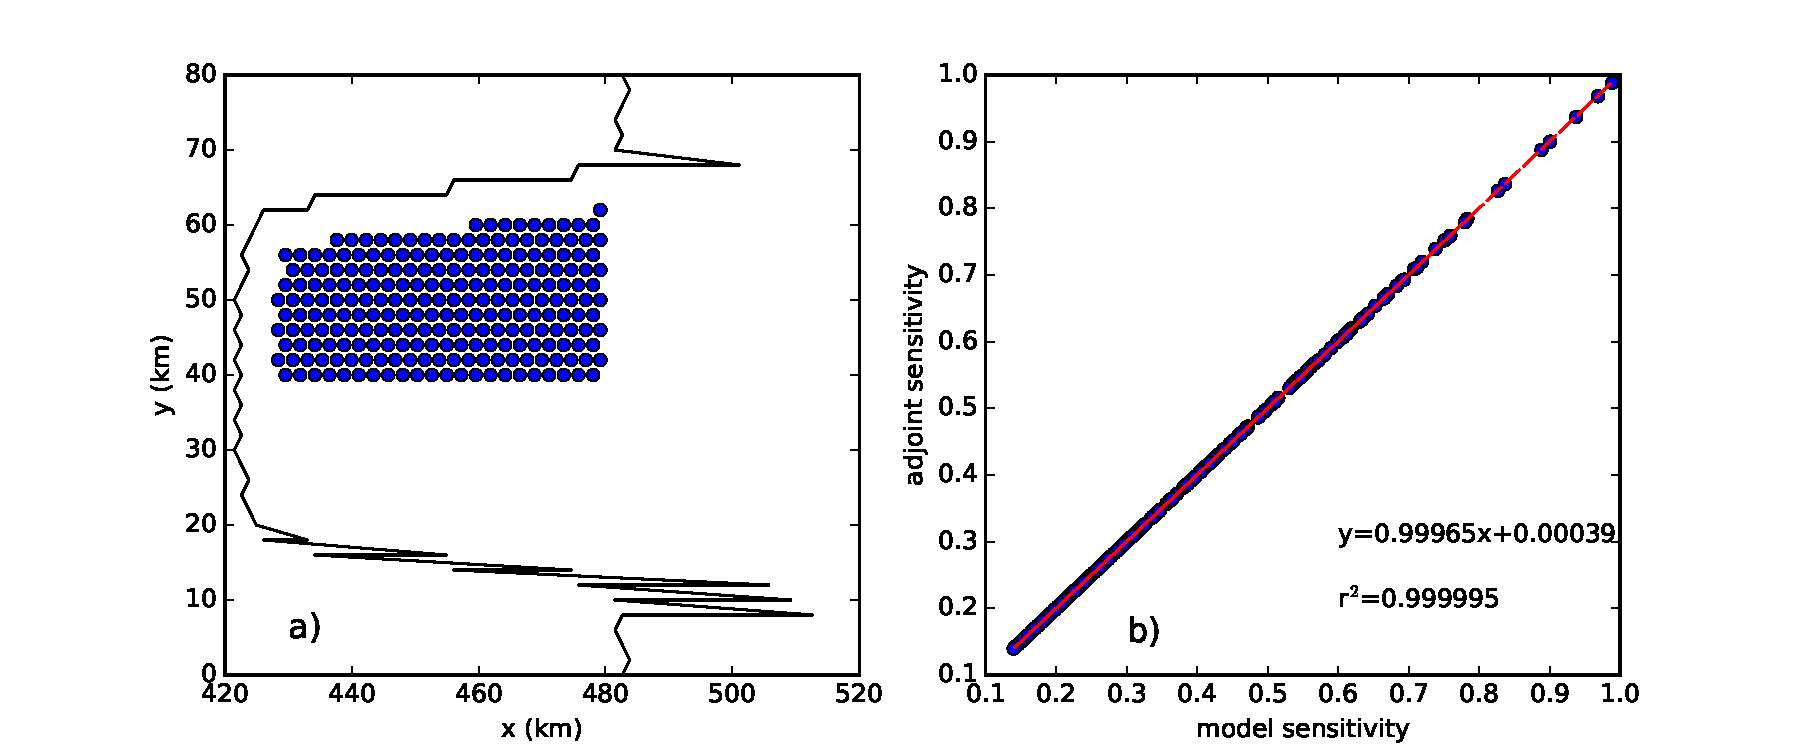
\includegraphics[width=1\linewidth]{figs/adjoint_comp.pdf}
    \caption{Grounding line flux sensitivity for the MISMIP+ domain calculated from individual perturbation experiments versus derived from a model adjoint (perturbation locations are shown by circles in a). Perturbation-experiment (x-axis) and adjoint-derived (y-axis) sensitivities (see text for definition) are plotted against one another in b). In a and b, the red circles indicate near-GL ($<$2 km) perturbation points, which are omitted in the comparison in b and d. The GL in a and c is shown by the black curve. In b and d, the red line is a linear regression between the perturbation-experiment and adjoint-derived sensitivities.}
	\label{adjoint_comp}
\end{figure}



%\subsection{MISMIP+}
%Before and after the perturbation, the GL velocity change clearly shows a spatial pattern (Fig \ref{stndVarFluxP}a). By calculating the standard deviation of the velocity change along GL for each 2 km perturbation experiment, we can see that the GL velocity change data is more dispersed for perturbation near GL, while for pertuirbations at the central region of the ice shelf, the corresponding GL velocity change is less variant along GL. If we look at Fig.~\ref{stndVarFluxP}b, the integrated GL flux is more contributed by the GL cells that close to the perturbation spot, i.e., the neighboring GL cells appears to have more flux contribution weight than those far away from the perperturbation location, and the perturbations near the ice shelf center tend to impact more uniformly on the GL dynamics.

%\begin{figure}
%\centering
%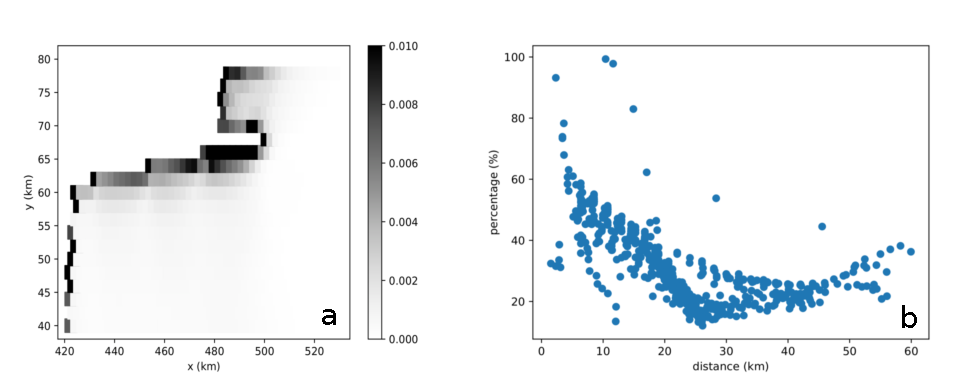
\includegraphics[width=1\linewidth]{figs/stndVarFluxP.pdf}
%\caption{(a) The distribution of the standard variance of the ice velocity changes on the grounding line of MISMIP+ for all perturbation experiments (note we only do the perturbation experiments for half space in $y$ of MISMIP+); (b) We find five cells on the grounding line that are the nearset to the perturbation spot. The x-axis is their mean distances to the perturbation box. The y-axis shows their combined flux contribution in the total integrated grounding line flux.}
%\label{stndVarFluxP}
%\end{figure}

%This can be further examined by looking at the relationship between GL flux response number ($N_r$) and the buttressing number ($N_b$) for the first principal stress ($\sigma_{p1}$) at different $dG$ and $dC$ (Fig \ref{diffdCdG}). $dG$ ($dC$) is the minimum distance between perturbation boxes and GL (calving front). When both $dG$ and $dC$ increase, perturbation boxes are farther away from GL and calving front, the velocity changes at GL become less dispersible and their relationship gets less ``noisy'' and tends to show linear trends. The possible explanaions can be found in the following ``Discussions'' section.

%\begin{figure}
%\centering
%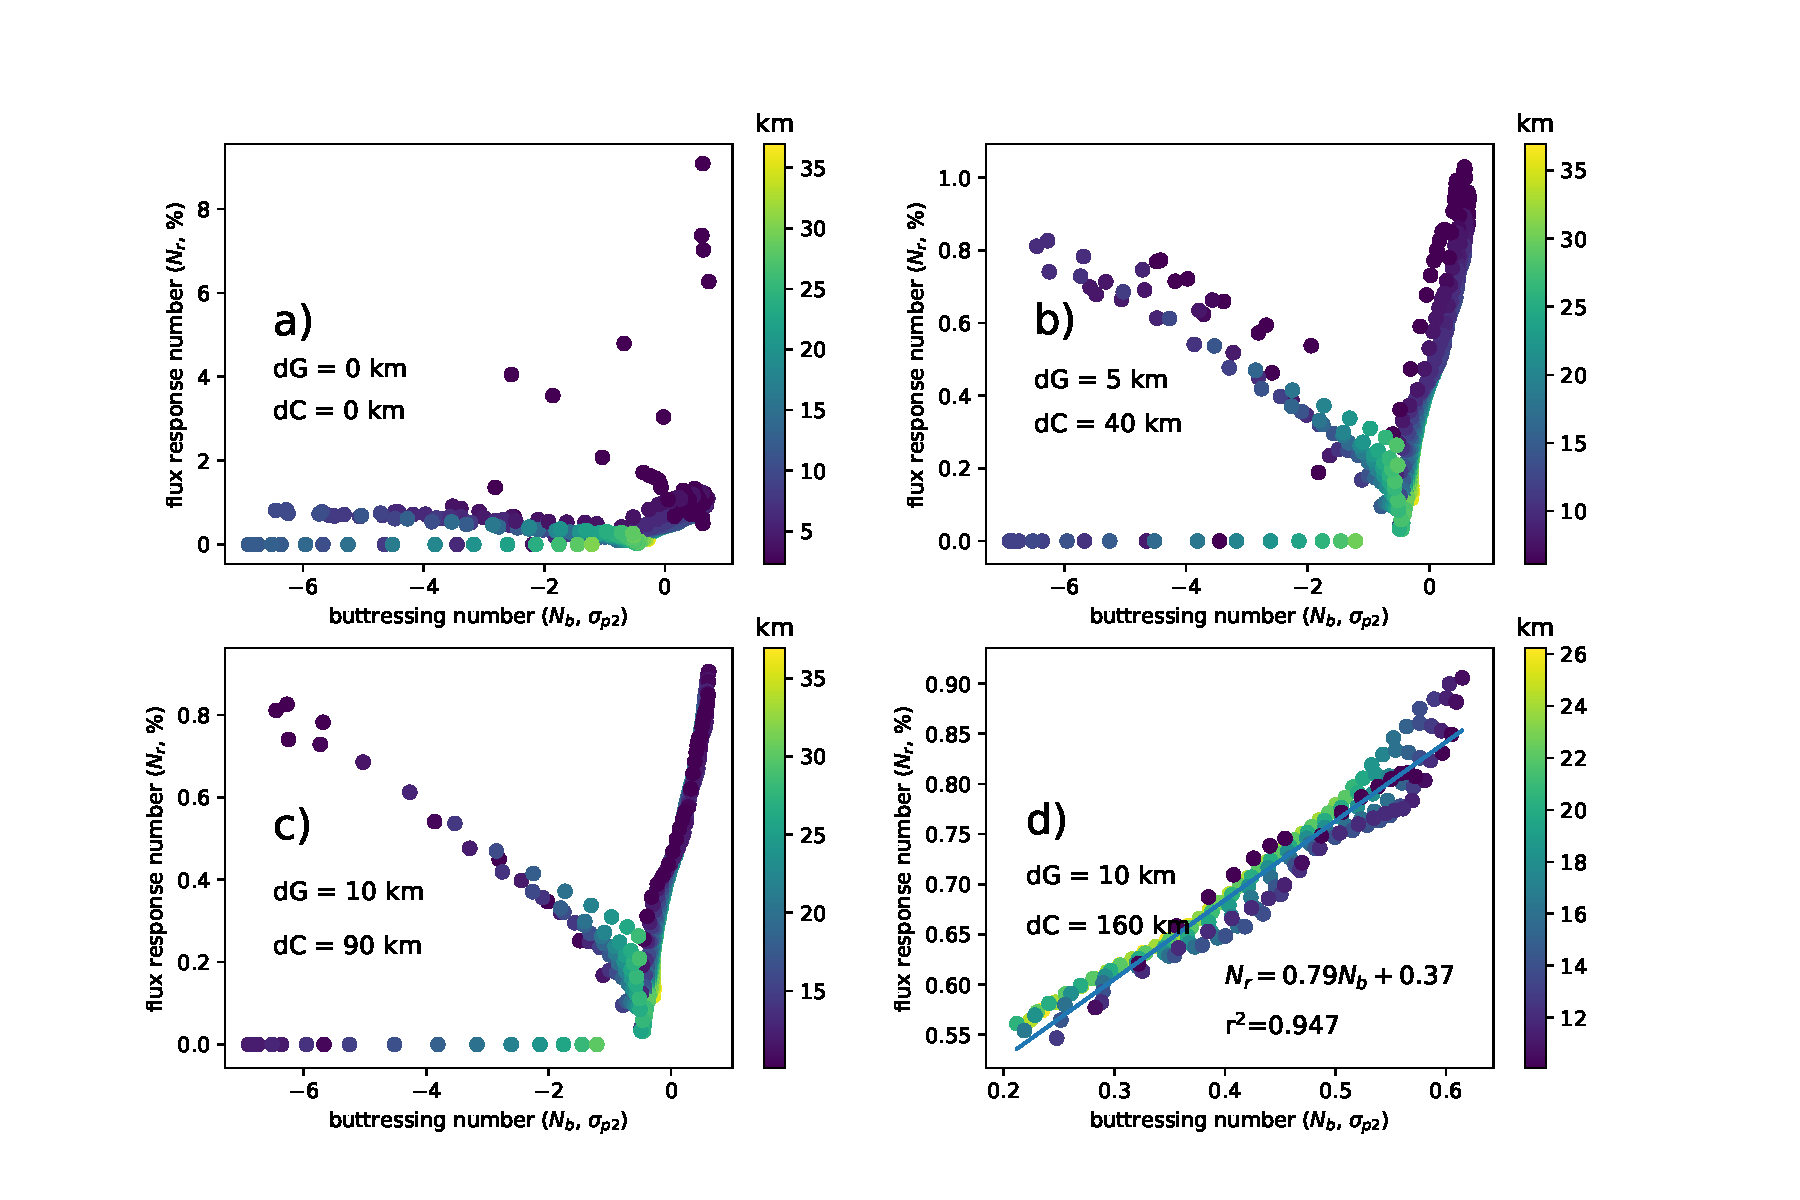
\includegraphics[width=1\linewidth]{figs/diffdCdG.pdf}
%\caption{The relationships between the groundling line flux response number ($N_r$) and the buttressing number ($N_b$) at the perturbation spots by different geometric filters of $dG$ and $dC$. Larger $dG$ and $dC$ give perturbation spots that are more centralized in the ice shelf. Smaller $dG$ and $dC$ mean the perturbation locations are either close to the grounding line or the calving front. The color bars show the values of $dG$ for each perturbation spot.}

%\label{diffdCdG}
%\end{figure}

%In fact, $\sigma_{p1}$ appears to be the best metric for predicting such linear relationship, comparing to the other 7 stress components (Fig \ref{diffStressComp}). The $N_b$ for $\sigma_f$, $\sigma_{af}$, $\sigma_x$ and $\sigma_y$ show some weak correlations with GL flux response number $N_b$. The shear stress and hoop stress, however, have no clear evidences of relating to $N_r$. Note that for all plots in Fig.~\ref{diffStressComp}, we have removed the ``noisy'' perturbation spots using $dG$ and $dC$. It is suprising that $\sigma_{p1}$ shows better performance than $\sigma_{p2}$ and $\sigma_s$, as $\sigma_{p2}$ gives the maximum buttressing number and predicts well the passive ice regions in \citet{furst2016} and the shear stress supply the main large resistence force for divergent ice flow regions (most of the MISMIP+ ice shelf) \citep{wearing2016}.

%\begin{figure}
%\centering
%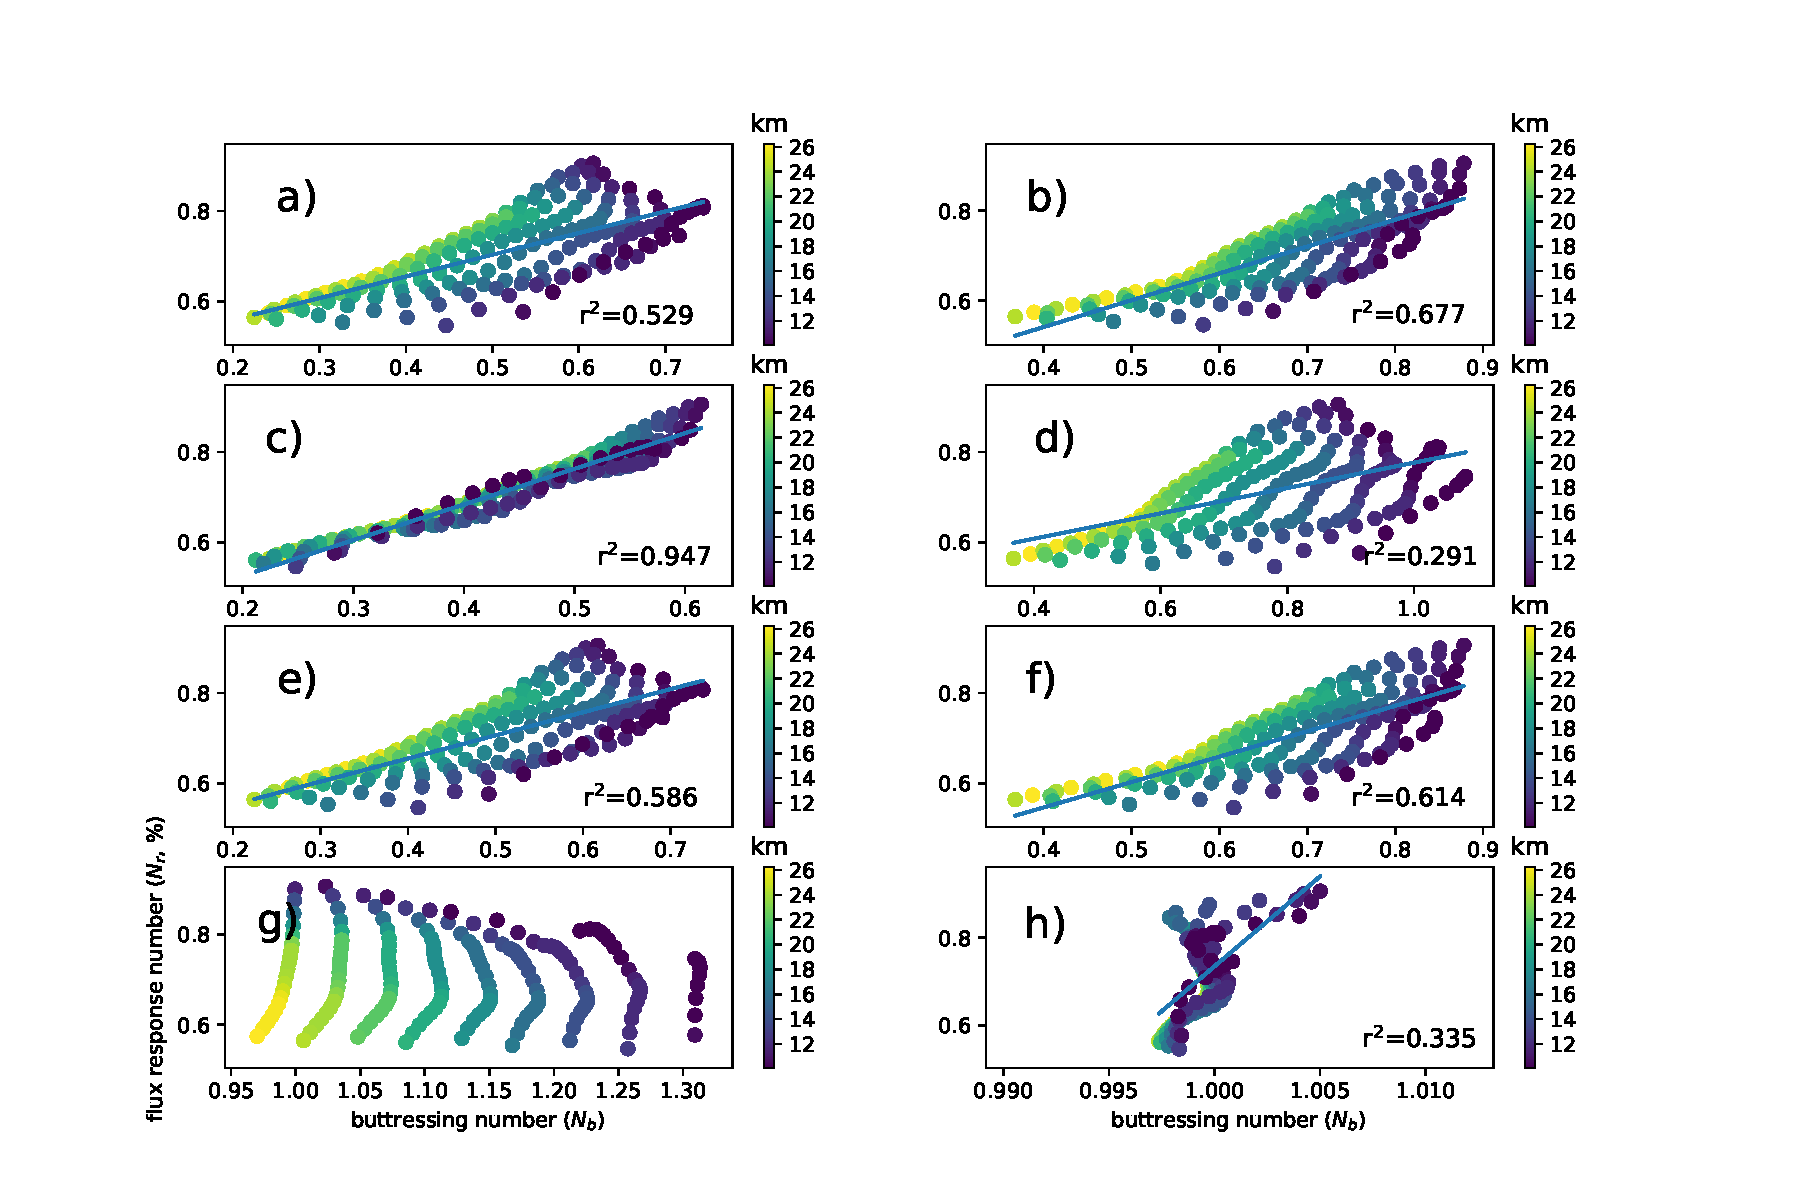
\includegraphics[width=1\linewidth]{figs/diffStressComp.pdf}
%\caption{The relationships between grounding line flux response number ($N_r$) and eight different stress components, $\sigma_f$ (a), $\sigma_{af}$ (b), $\sigma_{p1}$ (c), $\sigma_{p2}$ (d), $\sigma_{x}$ (e), $\sigma_{y}$ (f), $\sigma_{s}$ (g) and $\sigma_h$ (h). See Table \ref{stressDef} for the definition of each stress component in the MISMIP+ 2 km $\times$ 2 km box experiments. The color bars show the values of $dG$ for each perturbation spot.}
%\label{diffStressComp}
%\end{figure}

%The buttressing number for $\sigma_{p1}$ also performs well for the 10 km $\times$ 10 km square box perturbation experiments (Fig \ref{diffStressCompAvg}), for which we average the stresses across all cells in each square box. In fact, except the shear stress $\sigma_s$, all correlations are improved compared to the 2 km $\times$ 2 km perturbation experiments. In particular, the hoop stress shows some improved predictability as well. But again, $\sigma_{p2}$ is still not preferable than $\sigma_{p1}$.

%\begin{figure}
%\centering
%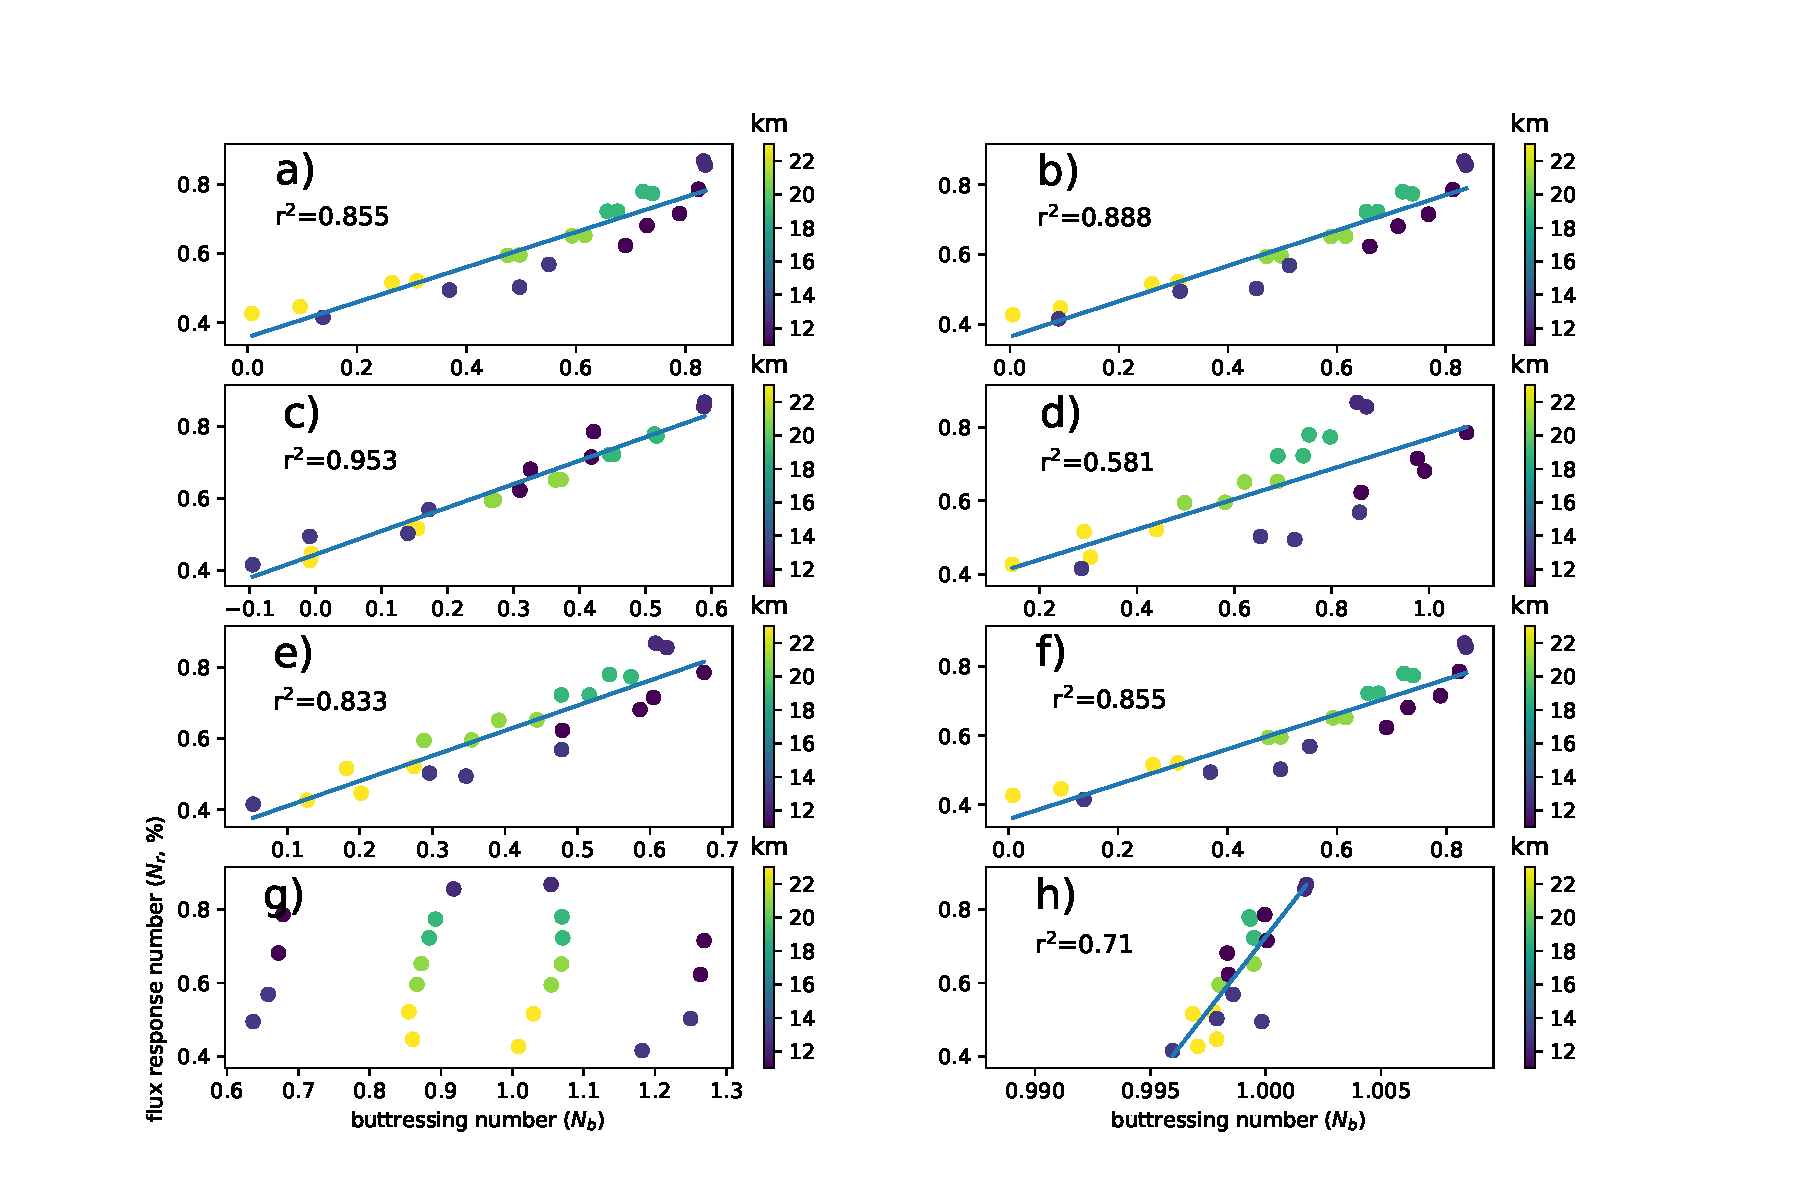
\includegraphics[width=1\linewidth]{figs/diffStressCompAvg.pdf}
%\caption{The relationships between grounding line flux response number ($N_r$) and eight different stress components, $\sigma_f$ (a), $\sigma_{af}$ (b), $\sigma_{p1}$ (c), $\sigma_{p2}$ (d), $\sigma_{x}$ (e), $\sigma_{y}$ (f), $\sigma_{s}$ (g) and $\sigma_h$ (h). See Table \ref{stressDef} for the definition of each stress component in the MISMIP+ 10 km $\times$ 10 km box experiments. The color bars show the values of $dG$ for each perturbation spot.}
%\label{diffStressCompAvg}
%\end{figure}


%\begin{figure}
%\centering
%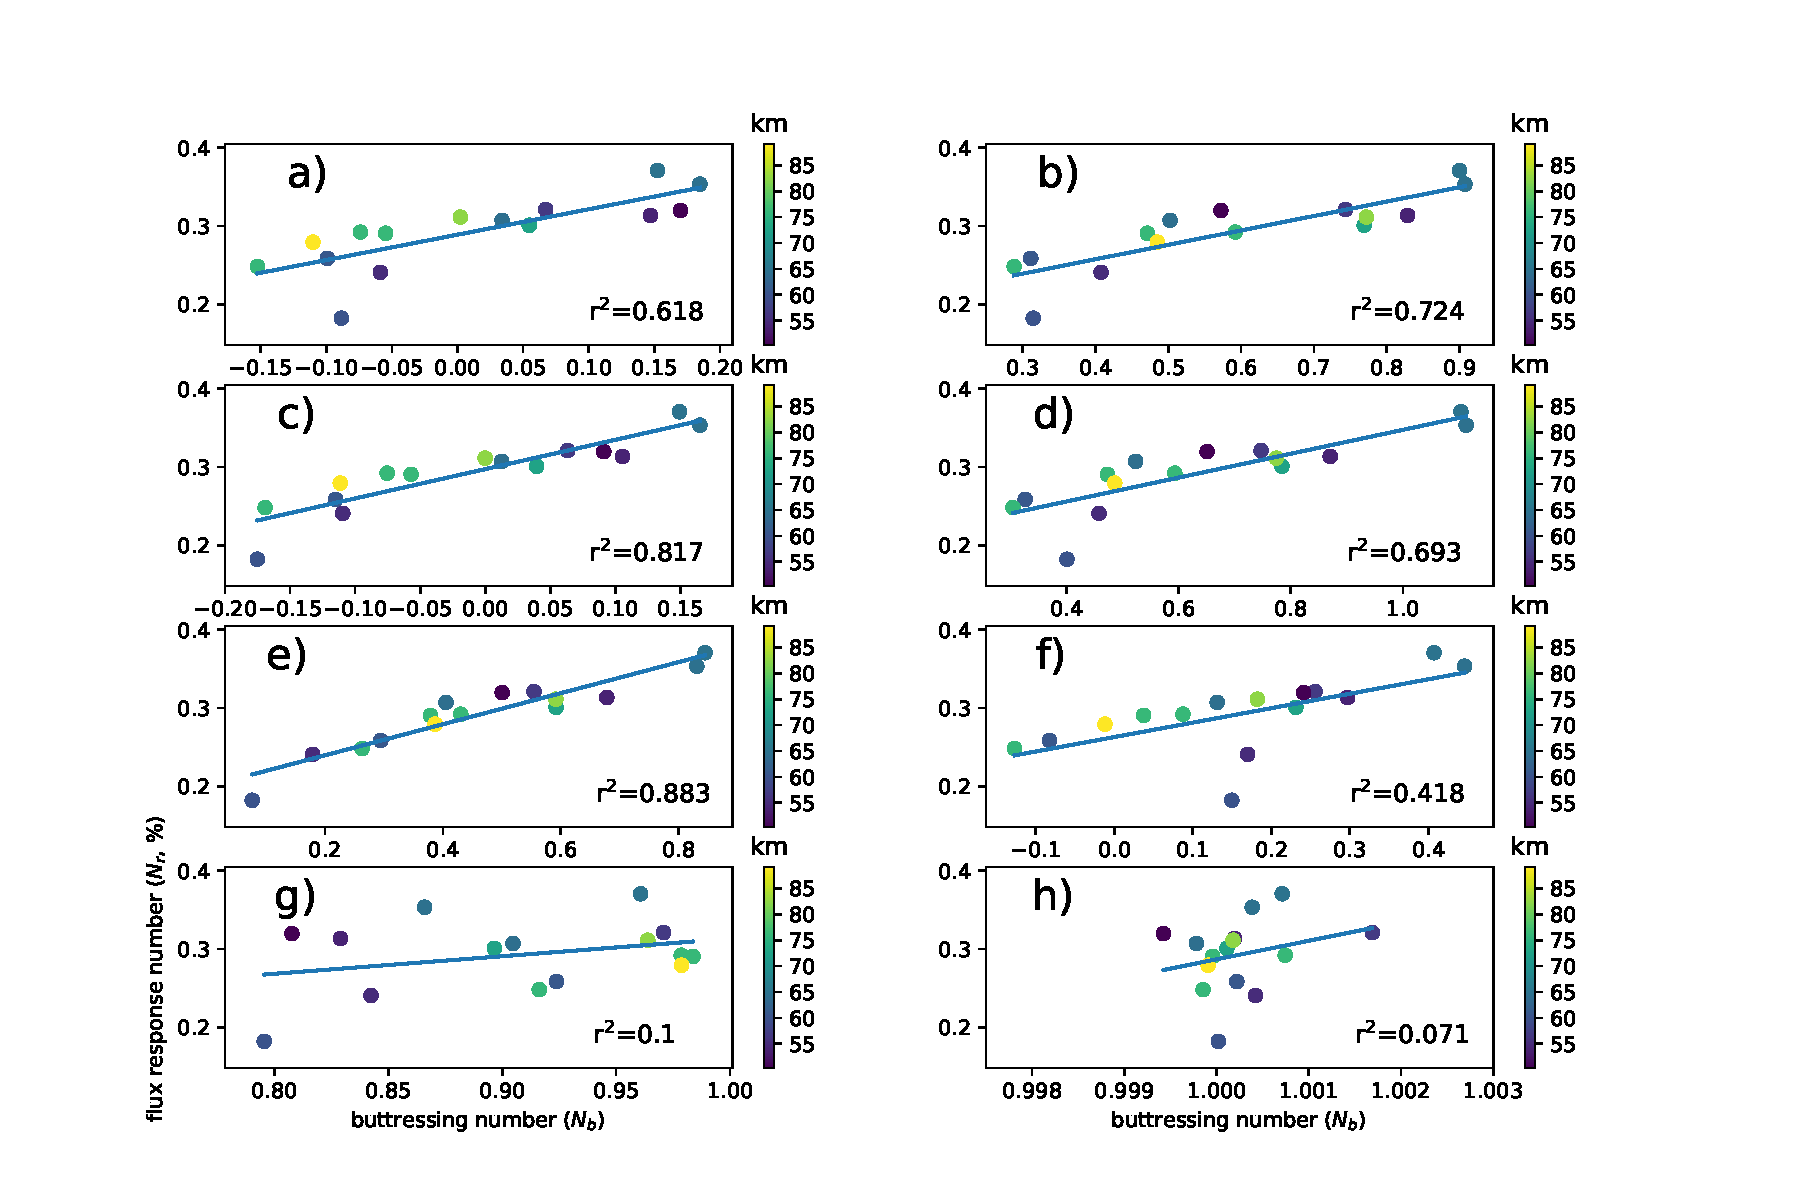
\includegraphics[width=1\linewidth]{figs/diffStressCompAvgL.pdf}
%\caption{The relationships between grounding line flux response number ($N_r$) and eight different stress components, $\sigma_f$ (a), $\sigma_{af}$ (b), $\sigma_{p1}$ (c), $\sigma_{p2}$ (d), $\sigma_{x}$ (e), $\sigma_{y}$ (f), $\sigma_{s}$ (g) and $\sigma_h$ (h). See Table \ref{stressDef} for the definition of each stress component in the Larsen C 20 km $\times$ 20 km box experiments. The color bars show the values of $dG$ for each perturbation spot.}
%\label{diffStressCompAvgL}
%\end{figure}

%Fig.~\ref{fig1} shows the relationships of integrated GL flux change and various buttressing numbers for different stresses for all perturbations over the MISMIP+ ice shelf. The inherent pattern is ambiguous. However, if we look closely to the distances of the perturbation points to GL, we can see the far scattered points are mostly near to the GL. Figure \ref{mismip_Nb_GLF_regression} is an example of the impact of perturbation location on the velocity changes across the ice shelf and on GL. In addition to the complex velocity change patterns around the perturbation location, there are two clear patterns we can find: 1) the magnitude of vel. change decreased with distances away from the perturbation and 2) the vel. change pattern is different when the perturbation approaches to the GL. 

%The first one is easy to understand as the energy of perturbation decreases when it propagate away to far upstream and downstream. The second one can be explained by at least two mechanisms: 1) ice dynamics are more remarkably impacted by the grounded ice flow near the GL and 2) the propagation of perturbation can be more impacted by the spatial GL geometry. These two impacts can be confirmed if we remove the perturbation points both near the GL and in the open ice shelf area (little buttressing). See Fig.~\ref{mismip_r2_all_direction}, we only keep the perturbation points that are > 5 km away from the GL and also their x coordinates are < km 480 and some clear trends starts to appear. The buttressing number for shear and hoop stress seems to be not good metrics, but there are some relationships for $\sigma_{p1}$, $\sigma_{p2}$, $\sigma_f$, $\sigma_{af}$, $\sigma_x$ and $\sigma_y$, especially for $\sigma_{p1}$. 

%This can be further verified if we apply the perturbation to a spatial box (20km by 20 km) and calculate the average stress field in each perturbation box, by which we can smooth out and decrease the impacts of distances on the GL flux responses (Fig \ref{perturb_theta_velchange}). the shear stress buttressing number is still a bad metric, but the averaged hoop stress turns out to become much better than the 2 km perturbation cell case. Other stresses along different directions also present better behaviors for GL flux responses.

%Based on the above MISMIP+ results, we apply the same approaches to Larsen C Ice Shelf. See Fig.~\ref{stressDiff_velDiff_GL_allPerturb}, though Larsen C has a more complex geometry compared to MISMIP+, it still show good linear relationship between the $\sigma_{p1}$ buttressing number and GL flux response. Different than the MISMIP+ runs, we remove the perturbation spots that are < 10km to the GL and calving front.



%\section{Discussions}
%
%Based on the above discussion we hypothesize that the two main factors controlling how a local perturbation in ice shelf thickness leads to changes in ice flux across the GL are 1) the distance between a perturbation location and the GL and 2) the first principal stress at the perturbation location. Figure \ref{distPerturbComp} shows an example of the impact of the perturbation location on the velocity changes across the ice shelf and GL. Despite the complex patterns of velocity change around the perturbation spot, we can see two clear features: 1) the magnitude of velocity change decreases with distances away from the perturbation spot and 2) the velocity change pattern becomes different and more disordering when the perturbation  approaches to GL. 
%
%
%The first feature is easy to understand because the energy of perturbation decays as it propagate away to far upstream and downstream. However, the perturbation propagation is not simply dependent on distance, but replies on the ice flow field. A complete perturbation propagation theory is necessary to describe/explain these small velocity changes across the ice shelf, however, it is beyond the scope of this study. The second one can probably be explained by two ice-flow mechanisms: 1) ice shelf dynamics are remarkably impacted by the grounded ice flow near the GL since it's a coupled system for grounded ice sheet and floating ice shelf and in MALI they is resolved as an integrated system as well; 2) the propagation of perturbation can be impacted by the spatial GL geometry. For example, the perturbation in Fig.~\ref{distPerturbComp}a can not directly impact the ice on the other side of the grounded peninsula in the same way as for it's neighboring cells.
%
%In addition, the impacts of distance can also be verified from the box averaging experiments (Fig.~\ref{diffStressCompAvg} and \ref{diffStressCompAvgL}). By smoothing out the stresses in the perturbation box, different distances to GL for each cells and their impacts in the perturbation box are also averaged, resulting in better linear $N_b$-$N_r$ relationships. This possibly indicates that those linear $N_b$-$N_r$ relationships can apply for realistic ice shelves, as in reality the basal melting always occurs in wide spatial regions.
%
%%These two impacts can be confirmed if we remove the perturbation points both near the GL and in the open ice shelf area (little buttressing). See Fig.~\ref{mismip_r2_all_direction}, we only keep the perturbation points that are > 5 km away from the GL and also their x coordinates are < km 480 and some clear trends starts to appear. The buttressing number for shear and hoop stress seems to be not good metrics, but there are some relationships for $\sigma_{p1}$, $\sigma_{p2}$, $\sigma_f$, $\sigma_{af}$, $\sigma_x$ and $\sigma_y$, especially for $\sigma_{p1}$. 
%
%It is still not very clear why the integrated GL flux change is strongly correlated to the first principal stress at the perturbation location than other stress components (especially the second principal stress). We can find some clues by looking at the difference of $\sigma_{p1}$, $\sigma_{p2}$, $\sigma_f$ and $\sigma_s$ along GL before and after applying the perturbation (Fig \ref{stressDiff}). Clearly, the distribution of the difference of $\sigma_{p1}$ across ice shelf is less disordering than that of $\sigma_{p2}$, $\sigma_{f}$ and $\sigma_{s}$. This indicates that the propagation of the perturbation for different stress components can be greatly varied in patial, which is probably the main reason of those different $N_b$-$N_r$ relationships for different stress components. A further evidence of this explanation can be found in Fig.~\ref{stressDiff_velDiff}, where we show the changes of veocity and stress components on GL. Clearly, the change of ice speeds at GL is more relevant to of $\sigma_{p1}$ and $\sigma_{f}$, compared to $\sigma_{p2}$ and $\sigma_{s}$. This possibly indicate that the changes of ice velocity under small basal perturbations may be more likely controlled by the changes of the stress components that are more aligned with ice flow directions.
%
%
%Therefore, we can find similar patterns for shear stress $\sigma_s$. The ice flow for most parts of MISMIP+ and Larsen C Ice Shelf are divergent, which in practical don't supply any buttressing to resist along flow. Since the hoop stress is quite small (Fig \ref{diffStressCompAvg}h and Fig \ref{diffStressCompAvgL}h), the main source of buttressing arises from the shear flow of ice shelf (assume the buttressing is proportional to the magnitude of $\sigma_{obj}$). This can be confirmed in \citep{furst2016} where we can clearly see that some non-passive (with buttressing) ice shelf are purely extensive regime. Similar to the case of $\sigma_{p2}$, the complex spatial propagation of the perturbed stress change from the perturbation spot to GL is a possible cause.
%
%
%
%
%%From Fig.~\ref{mismip_Nb_GLF_regression} we can see the ice vel. change over ice shelf and GL depends on the relative location to GL position. When p is near the center of the ice shelf, the ice flux change is more predictable than p close to the GL. The magnitude of vel. change decrease with distance, and the vel. upstream (downstream) tends to show an increase (decrease). For the ice shelf (GL) upstream to the perturbation, a decrease of ice thickness indicates a decrease of buttressing, however, for ice shelf downstream to the perturbation, it means a decrease of driving stress. This pattern become ambiguous when the perturbation is close to GL as it's dynamics is more affected by the grounded ice sheet. 
%
%
%Though there is no clear linear $N_b$-$N_r$ relationships near GL, the integrated GL flux mainly depends on the GL flux of cells that are close to the perturbation spot. From Fig.~\ref{stndVarFluxP}b, we can see that for perturbations near GL, their impacts are mainly local and thus can only affect their neighboring ice streams, which can possibly enhance the spatial heterogeneity of marine ice sheet responses under ocean warming forcings.  


\conclusions

%\textbf{SP: A few notes from Steve on some points we want to make sure to review / discuss in this section:}

%\begin{enumerate}
%    \item revisit questions posed in final paragraph of intro section and briefly answer them (assuming those answers are supported by the work in the body of the paper), or if we don't answer them, replace them in the intro w/ questions we do / can answer
%    \item Summarize our thoughts on the use of a buttressing number based on p1 vs. p2 for analyzing ice shelves. For p1, we can show there's a clear relationship between increasing buttressing number and increasing sensitivity of GLF; for p2, we cannot show that is the case---GLF appears to be possibly a multivalued function of buttressing number (we could add the p2 buttressing number vs. GLF plot, as in figure 2, to appendix to support this). 
%    \item What can we say about previous papers based on our analysis here? Furst et al. use buttressing number based on p2, but here we show that this does not correlate well (for idealized or realistic shelves) w/ sensitivity to changes in GLF (Reese paper). So at least in terms of trying to connect some of the important ideas in those two papers (calculating a metric for buttressing strength and how buttressing changes lead to changes in GLF), we have pointed something potentially useful out (p1 is more relevant than p2). 
%    \item Summarize our thoughts on diagnosing GLF sensitivity to ice shelf buttressing for realistic ice shelves during simulations---adjoint method would probably be best as it's consistent w/ Reese et al. (gives us information on what parts of an ice shelf will have an impact on changes in GLF) but w/o associated cost of point-by-point perturbation approach.
%    \item In absence of adjoint, our metrics here (p1-based buttressing number) could still be of use for identifying areas that control changes in GLF ... but the area where they are useful / dependable over may be limited, and furthermore, it may be hard to know exactly how to define that area. (thus, it will be hard to have adequate confidence in using them)
%\end{enumerate}

%Among the main uncertainties and questions in the current ``hot spot''---Marine Ice Sheet Instability problem, the interactions between ice shelf and ocean are gaining increased interests in the glaciology community. 
There has been much recent and intense interest in the marine ice sheet instability (MISI), primarily in the context of the potential ongoing and future unstable retreat of sectors of the West Antarctic ice sheet (add REFS?). Due to the connections between ice shelf buttressing and the MISI, attention has shifted to better understanding the sensitivity of GLF to ice shelf basal melting. Specifically, where are ice shelves most vulnerable to basal melting in the context of increased GLF and can we predict the sensitivity of changes in GLF to ice shelf melting based on the present-day geometry and flow field of the ice shelf? In this study, we have attempted to address these questions, with the following findings:

The GLF response to thickness perturbation is highly dependent on the direction of buttressing. Although, locally, the buttressing is maximum along the second principal stress ($\sigma_{p2}$ direction, we find a much better correlation between GLF response to the buttressing defined in terms of the first principal stress ($\sigma_{p1}$) at perturbation points that are located near the center region of the ice shelf. The buttressing number (along $\mathbf{n}_{p2}$ and $\mathbf{n}_f$) approach adopted in \citet{furst2016} for identifying passive ice regions doesn't properly apply in terms of finding sensitive ice shelf regions that well connect basal melting and GLF responses.\textit{SP: We can hit this a little bit harder by pointing out that this is in disagreement with the work of Furst et al., who use sigma p2 to identify regions of passive ice.} \textit{Tong: I add a sentence here}  We argue that this is because the GLF response is controlled by both the dynamics at GL and the perturbation points and their relationship (for example, (13)) in between. Therefore, we cannot easily predict GLF response by only analyzing the geometric and dynamic features of a local perturbation, i.e, large basal melting at a location of high buttressing (large buttressing number along the $\sigma_{p2}$ direction) do not always lead to large GLF increases.

Near the GL, there is no clear connection between the buttressing at the perturbation points and the response of GLF, as 1) the pattern of ice flow across GL may be highly heterogeneous in space for real ice shelves and 2) the propagation of perturbation will be strongly affected by the local GL geometry. In this case, the distance between the perturbation point and GL may be playing the critical role, as the energy of the perturbation decays over distance. We observe large increase of ice speed and flux for GL cells that are close to the perturbation points. This indicates two possible consequences: 1) the grounded ice sheet dynamics will be negligibly affected if the GL dynamics is insensitive to melt perturbation (e.g., the bed topography is downward sloping or the ice thickness at GL is thin); 2) the retreats of GL will be spatially heterogeneous if the dynamics of local GL is sensitive to the perturbation (e.g., the bed topography has retrograde slope and large ice thickness) while the remote portion of GL experience relatively little impact from the perturbation.

Considering the complex pattern of the connection between GLF response and buttressing number at perturbation points for real ice shelves, we propose to adopt the adjoint sensitivity method in the ice sheet model to accurately capture the dynamic change of GLF sensitivities. For perturbation points that are near to the (can we say something quantitative here, like using the thickness gradient metric?) GL, the adjoint method may not provide consistent results due to the large gradient of ice geometry (nonlinearity), but it can capture the complex ice dynamics along GL for real ice shelves for most perturbation points. By introducing the adjoint sensitivity method we do not need to do every perturbation experiment to determine the sensitivity map of an ice shelf. \textbf{TZ: I think we need further evidence of adjoint ability on complex real ice shelves. What do you think, Steve? SP: I'm inclined to see if we can get away with it for now, and only address it if we are asked for it in review.}

For ice-sheet models that lack an adjoint capability, our anaylisis here can also provide a rough guide to determine the sensitivity of GLF to basal melt at different locations on the ice shelf (e.g. use a metric like (13) to find the dominant buttressing direction and compare the buttressing number values at different perturbation points). But we acknowledge that it is a somewhat arbitrary choice to remove those perturbation points that are near GL and calving front.

%The sensitivity analysis presented in this study are based on small (1 m) thickness perturbations, same as previous studies like \citet{reese2018} . However, it's still unclear if they can still hold for large melts at values. Despite the progress we have made in this study, we suggest to apply a fully-developed perturbation propagation model for further understanding the physics of GL flux changes under ocean forcings. 

%From this study we find that the sensitivity of grounding line (GL) flux to melt perturbations beneath ice shelves appears to be linearly related to the buttressing number for certain stress field of the ice flow regime when the perturbations are located near the center of ice shelves. We can divide an ice shelf into three different geometric regions: 1) near GL where the shear margins dominate; 2) near the calving fronts where ice can be considered as ``passive'' and 3) the central regions of ice shelf. Though it is ambiguous to indentify the boundaries of those three sub-regions, we find that both the shear margins and passive ice regions show very weak linear connections to GL flux changes. The shear margins are strongly impacted by the upstream grounded stream flows and the passive ice shelf basically has negligible contribution to GL dynamics. 

%The buttressing of ice shelf resists ice flows from upstream. The maximum buttressing number (calculated from the second principal stress $\sigma_{p2}$) is a commonly used metric to quantify the buttressing effects of ice shelf, doesn't show clear correlations to the changes of GL flux. Among many possible factors we find that the distance away from perturbation locations may be a critical control for perturbation propagation across ice shelves, which is important for understanding the relationships between the stress field of the ice shelf and the GL flux changes. The GL ice speed changes may be more correlated to the changes of the first principal stress ($\sigma_{p1}$) and normal stress along flow ($\sigma_{f}$) than other stress components, for example, the second principal stress ($\sigma_{p2}$) and the shear stress ($\sigma_s$), indicating that the stress component ($\sigma_{p2}$) that contribute significantly to buttressing is not necessarily related to the progapation of buttressing. 

%The linear $N_b$-$N_r$ relationships presented in this study are based on small (1 m) thickness perturbations. However, it's still unclear if they can stand for large melts at the bottom of ice shelves ({\bf{Perhaps we also need to do large perturbation experiments?}}). Despite the progress we have made in this study, we suggest to apply a fully-developed perturbation propagation model for further understanding the physics of GL flux changes under ocean forcings. 

\section{Acknowledgements}
Support for this work was provided through the Scientific Discovery through Advanced Computing (SciDAC) program funded by the US Department of Energy (DOE), Office of Science, Biological and Environmental Research, and Advanced Scientific Computing Research programs. This research used resources of the National Energy Research Scientific Computing Center, a DOE Office of Science user facility supported by the Office of Science of the US Department of Energy under contract no. DE-AC02-05CH11231.

\bibliographystyle{copernicus}
\bibliography{refs}


\appendix

\section{Appendix materials}
%\renewcommand\thefigure{\thesection.\arabic{figure}}  
\renewcommand{\thefigure}{A\arabic{figure}}
\setcounter{figure}{0}

\begin{figure}
	\centering
	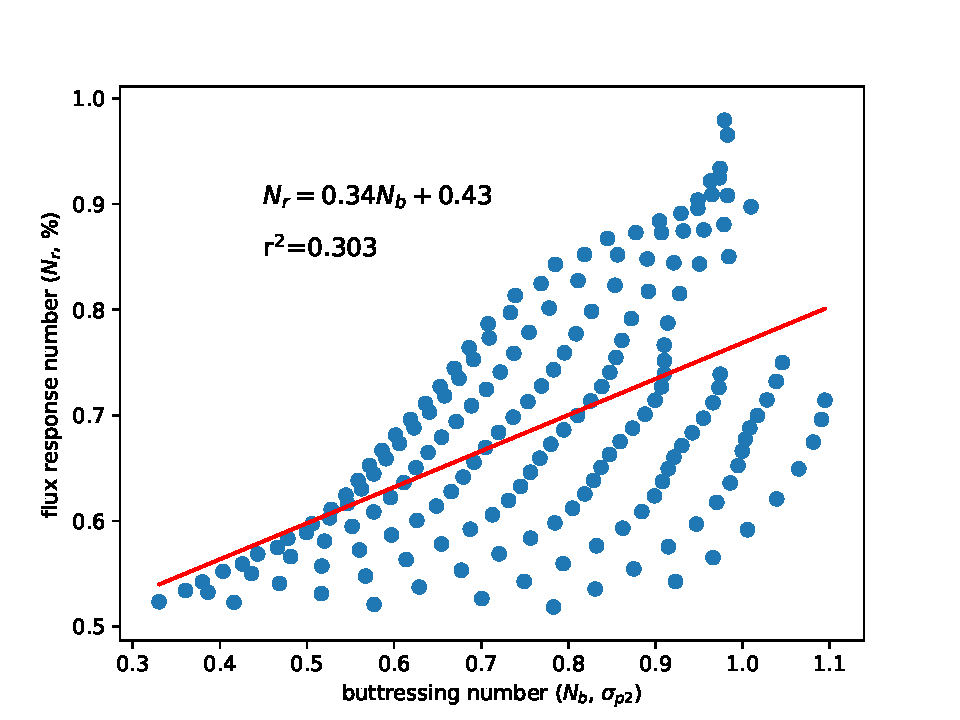
\includegraphics[width=1\linewidth]{figs/sigma_p2_example.pdf}
	\caption{$N_b$:$N_r$ correlation for perturbation points within the confined region of the shelf and with a thickness gradient magnitude $\left|\nabla H\right|<7$x$10^{-3}$. $N_b$ is calculated from the second principal stress $\sigma_{p2}$.}
	\label{sigma_p2_example}
\end{figure}

\begin{figure}
	\centering
	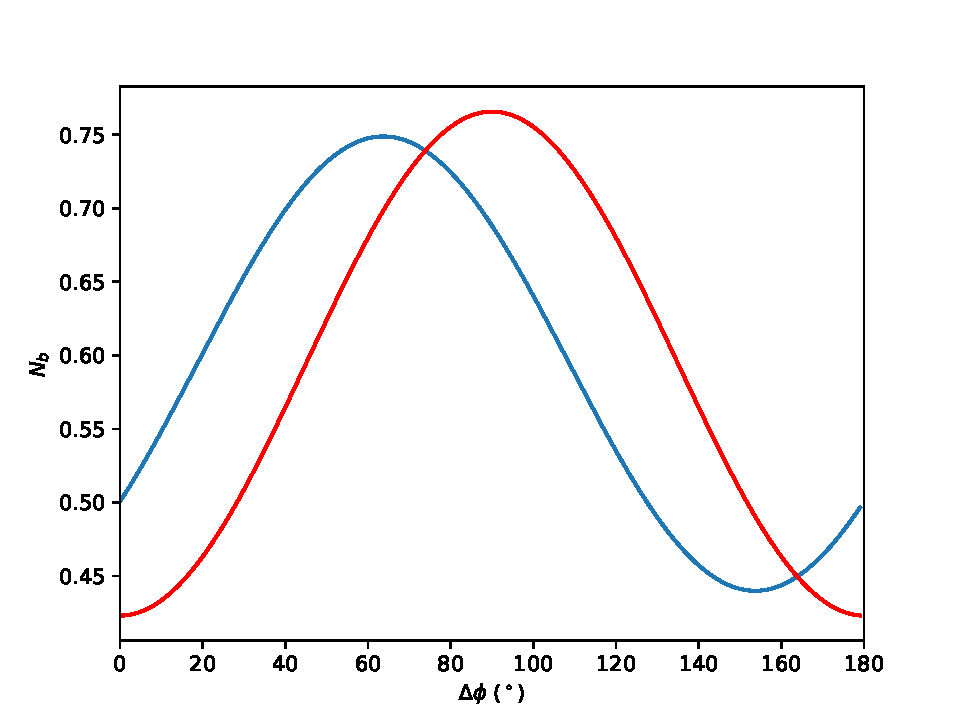
\includegraphics[width=1\linewidth]{figs/Nb_Deltaphi.pdf}
	\caption{$N_b$ values rotated counterclockwise by $\Delta\phi$ degrees relative to the $\sigma_{p1}$ direction (red) and the ice flow direction (blue). It's a twin plot for Fig.~\ref{mismip_Nb_GLF_regression}a. Both curves show the buttressing number is largest along the $\sigma_{p2}$ direction.}
	\label{Nb_Deltaphi}
\end{figure}

\begin{figure}
	\centering
	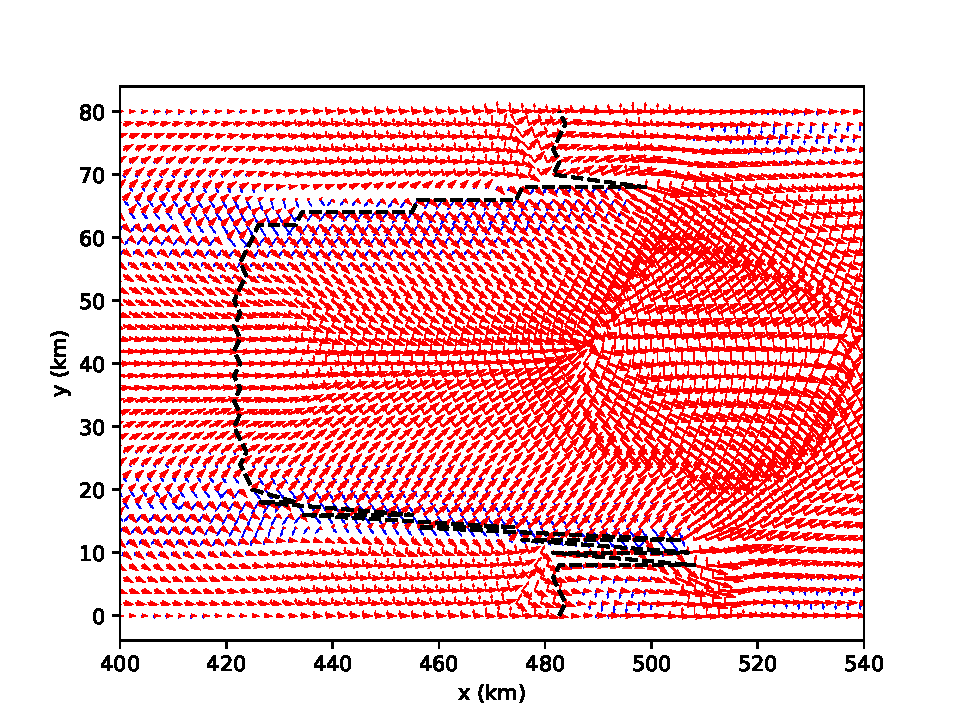
\includegraphics[width=1\linewidth]{figs/principal_stress_quiver.pdf}
	\caption{The quiver plot of $\sigma_{p1}$ (thick arrows) and $\sigma_{p2}$ (thin arrows) field. The red and blue colors means tensile and compressive stress, respectively. The thick dashed black line represents the grounding line.}
	\label{principal_stress_quiver}
\end{figure}

\begin{figure}
 	\centering
     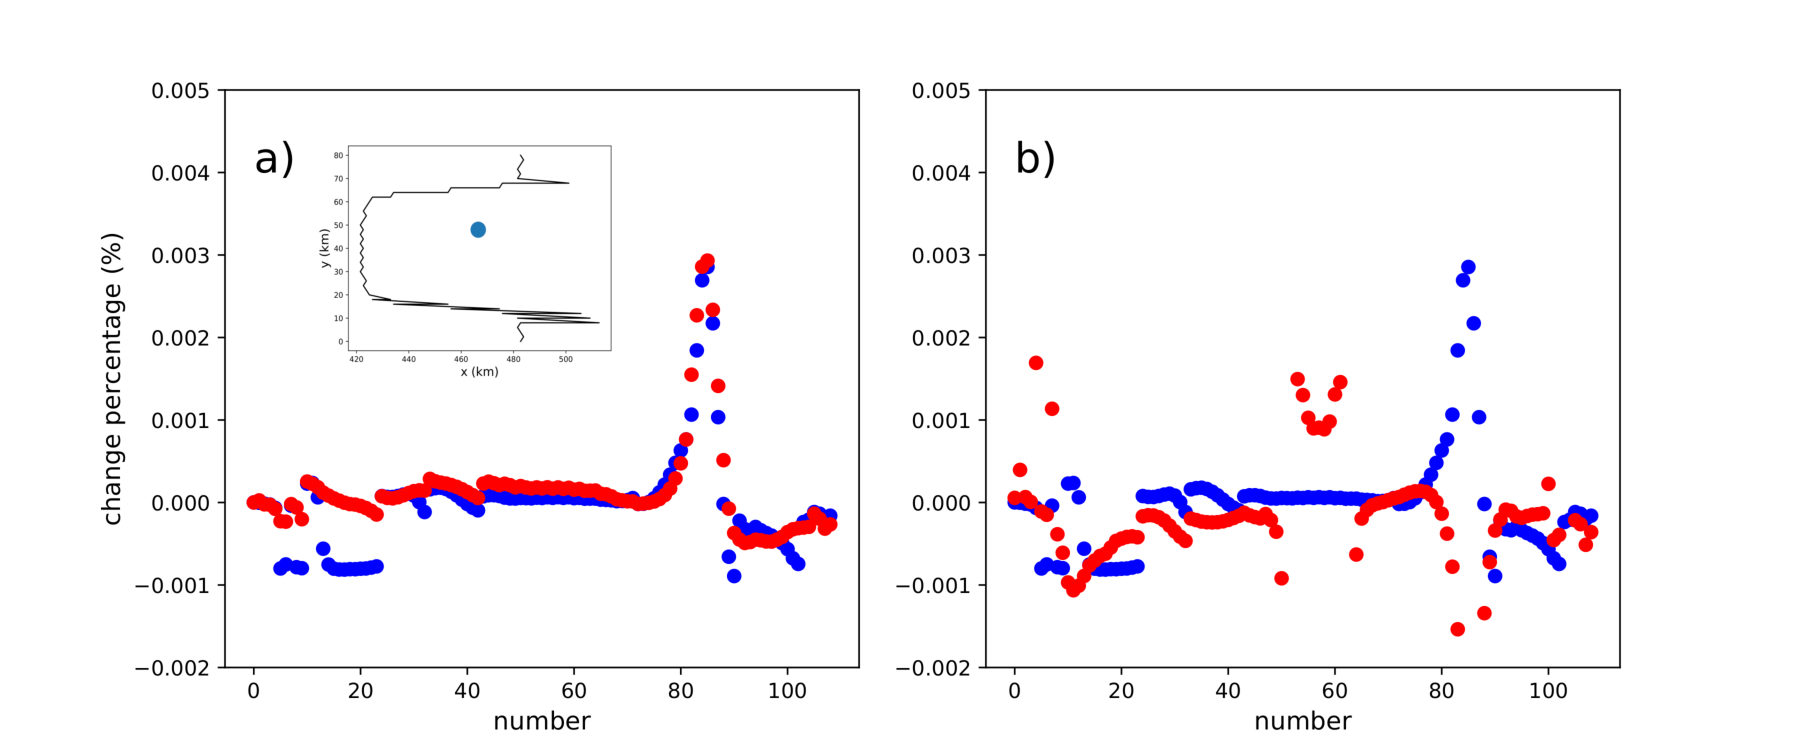
\includegraphics[width=1\linewidth]{figs/vel_stress_change_example.pdf}
     \caption{Relationship between changes in velocity (blue) and changes in the stress (red) along the GL for the MISMIP+ test case, due to a perturbation at a specific location on the ice shelf (blue dot in inset map). In a), changes in GL velocities are plotted against changes in $\sigma_{p1}$. In b), changes in GL velocity are plotted against changes in $\sigma_{p2}$. The $x$-axis represents an index for the grid cell number along the GL.}
 	\label{vel_stress_change_example}
\end{figure}

\begin{figure}
	\centering
	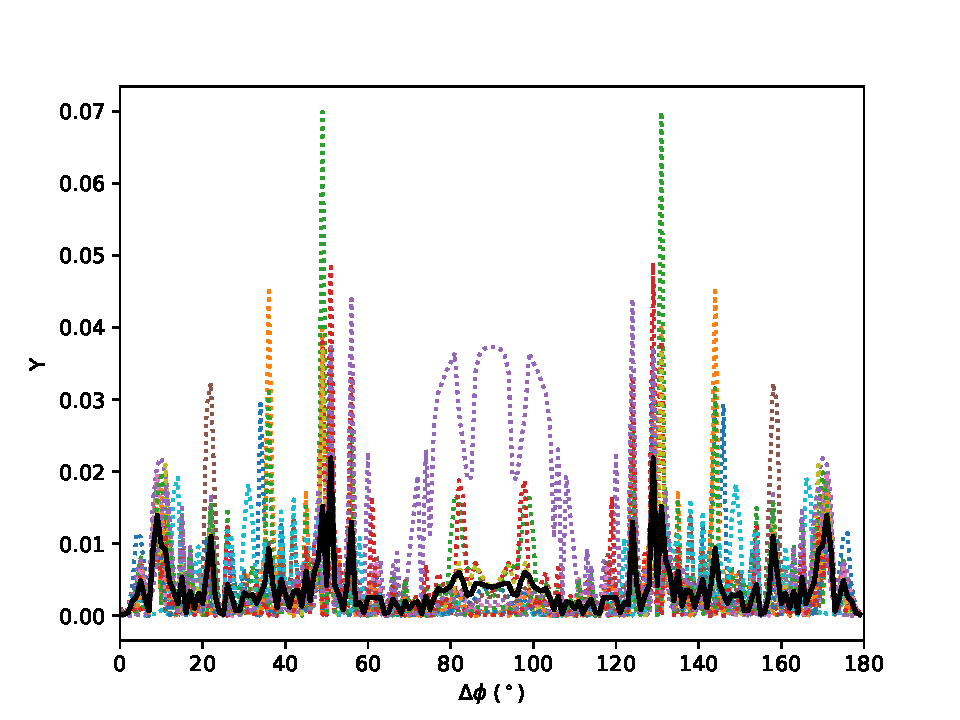
\includegraphics[width=1\linewidth]{figs/stress_vel_corr_GL_allP_larsenC.pdf}
	\caption{The correlation ($\Upsilon$) between the changes of ice surface speed and the changes of normal stress along GL for the Larsen C experiments. The direction of normal stress is rotated counterclockwise from the direction of $\sigma_{p1}$. The colored dashed curve each represents a perturbation experiment, and the thick back curve is their mean value.}
	\label{stress_vel_corr_GL_allP_larsenC}
\end{figure}

\begin{figure}
	\centering
	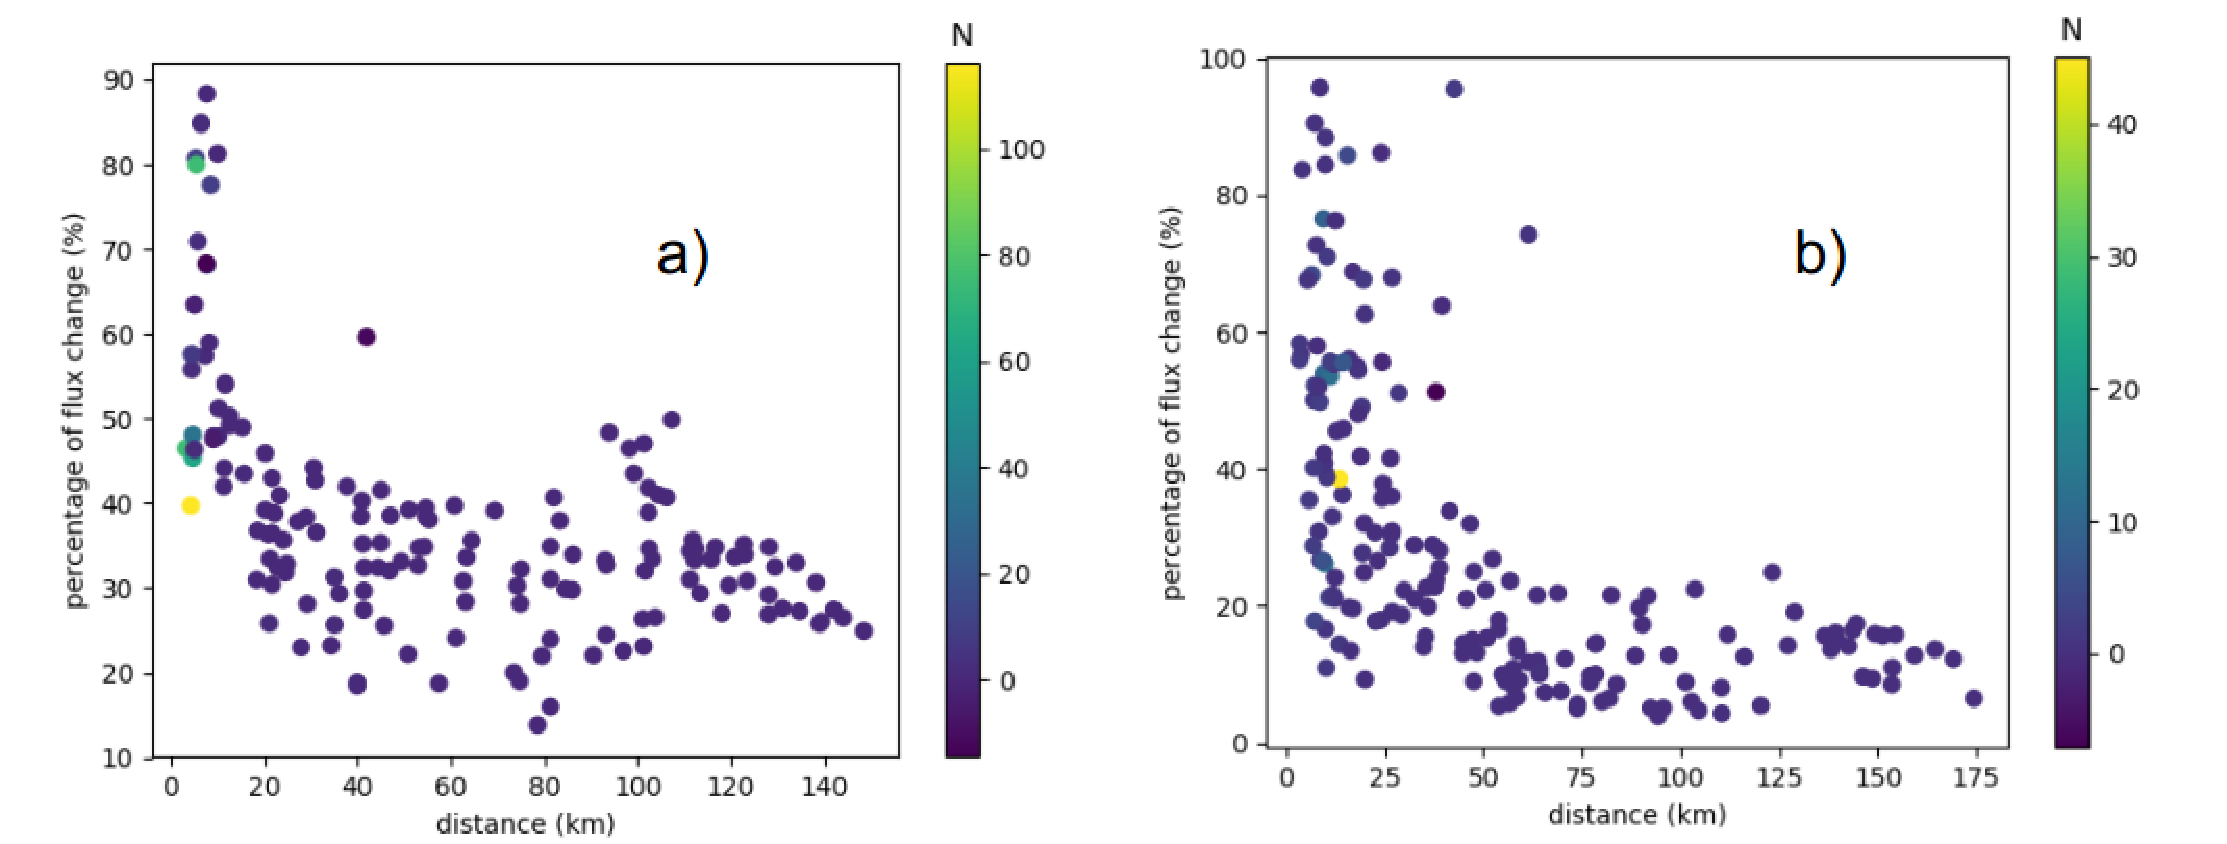
\includegraphics[width=1\linewidth]{figs/mismip_larsenc_dist.pdf}
	\caption{At each perturbation point, we locate the 5 closest GL cells and calculate the percentage ($y$-axis) of the total GL flux due to those 5 cells for a) MISMIP+ and b) Larsen C. The $x$-axis is the distance between the perturbation point and those 5 cells. The percentage is largest when the distance between the GL and the perturbation is small, supporting the concept that perturbations near the GL, in general, have a larger impact on the nearby flux across the GL. The colorbar shows the buttressing number.}
	\label{mismip_larsenc_dist}
\end{figure}

\begin{figure}
	\centering
	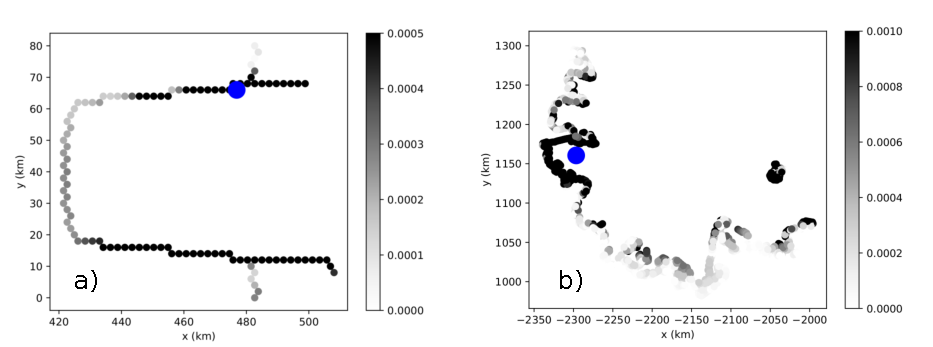
\includegraphics[width=1\linewidth]{figs/mismip_larsenC_velChange.pdf}
	\caption{The ice surface speed change (\%) along grounding line under certain specified perturbation locations for MISMIP+ (a) and Larsen C (b).}
	\label{mismip_larsenC_velChange}
\end{figure}

\begin{figure}
	\centering
    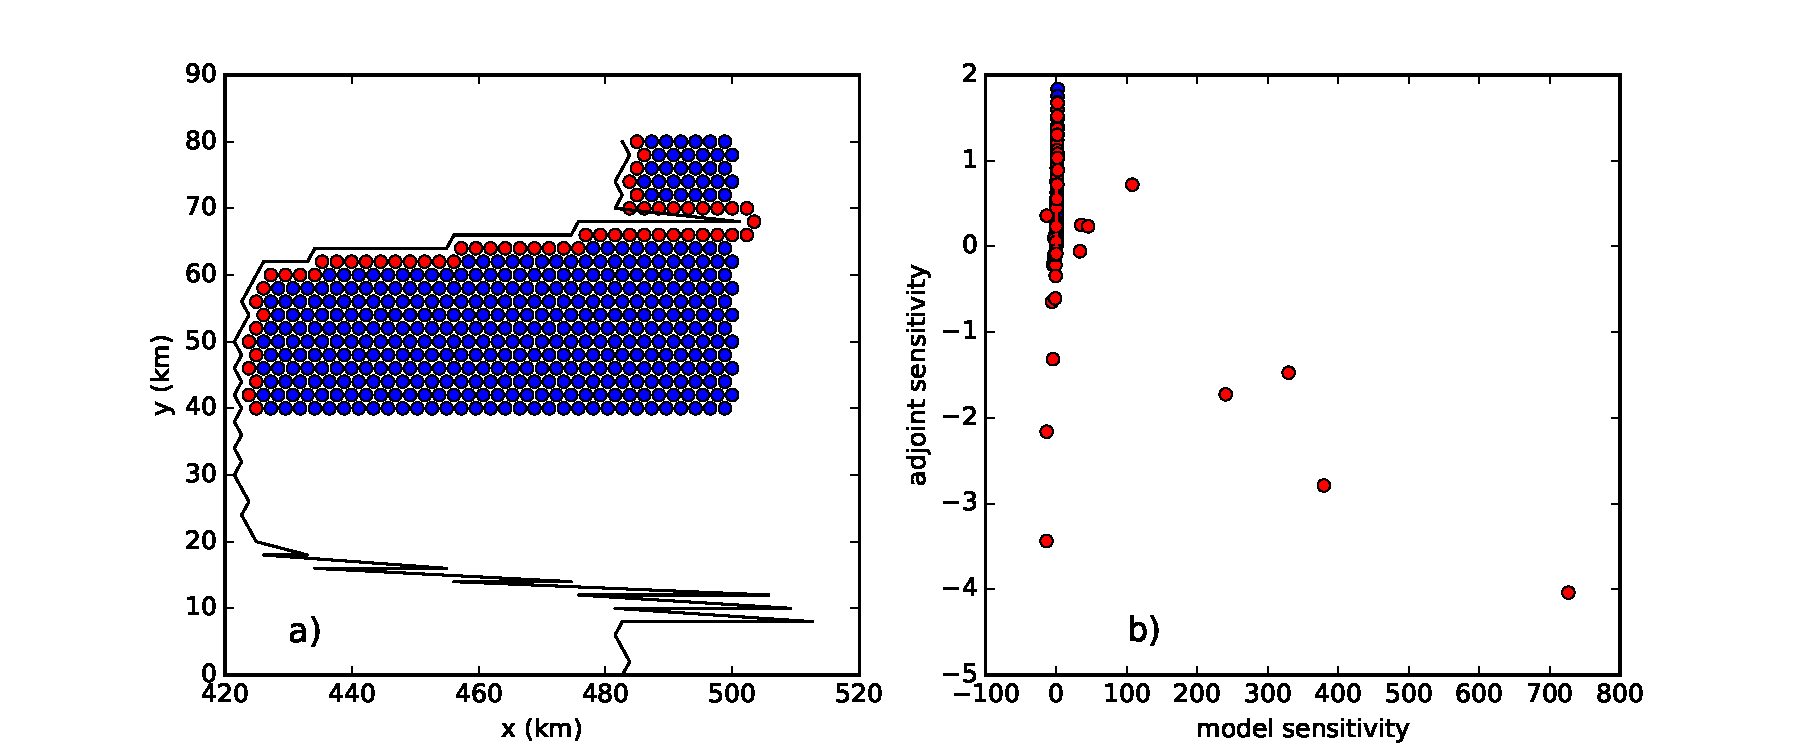
\includegraphics[width=1\linewidth]{figs/adjoint_comp_appendix.pdf}
    \caption{Grounding line flux sensitivity for the MISMIP+ domain calculated from individual perturbation experiments versus derived from a model adjoint (perturbation locations are shown by circles in a). Perturbation-experiment (x-axis) and adjoint-derived (y-axis) sensitivities (see text for definition) are plotted against one another in b). In a and b, the red circles indicate near-GL ($<$2 km) perturbation points, which are omitted in the comparison in Fig.~\ref{adjoint_comp}. The GL in a) is shown by the black curve. In b), the red line is a linear regression between the perturbation-experiment and adjoint-derived sensitivities.}
	\label{adjoint_comp_appendix}
\end{figure}



\noappendix

%\begin{figure}
%	\centering
%	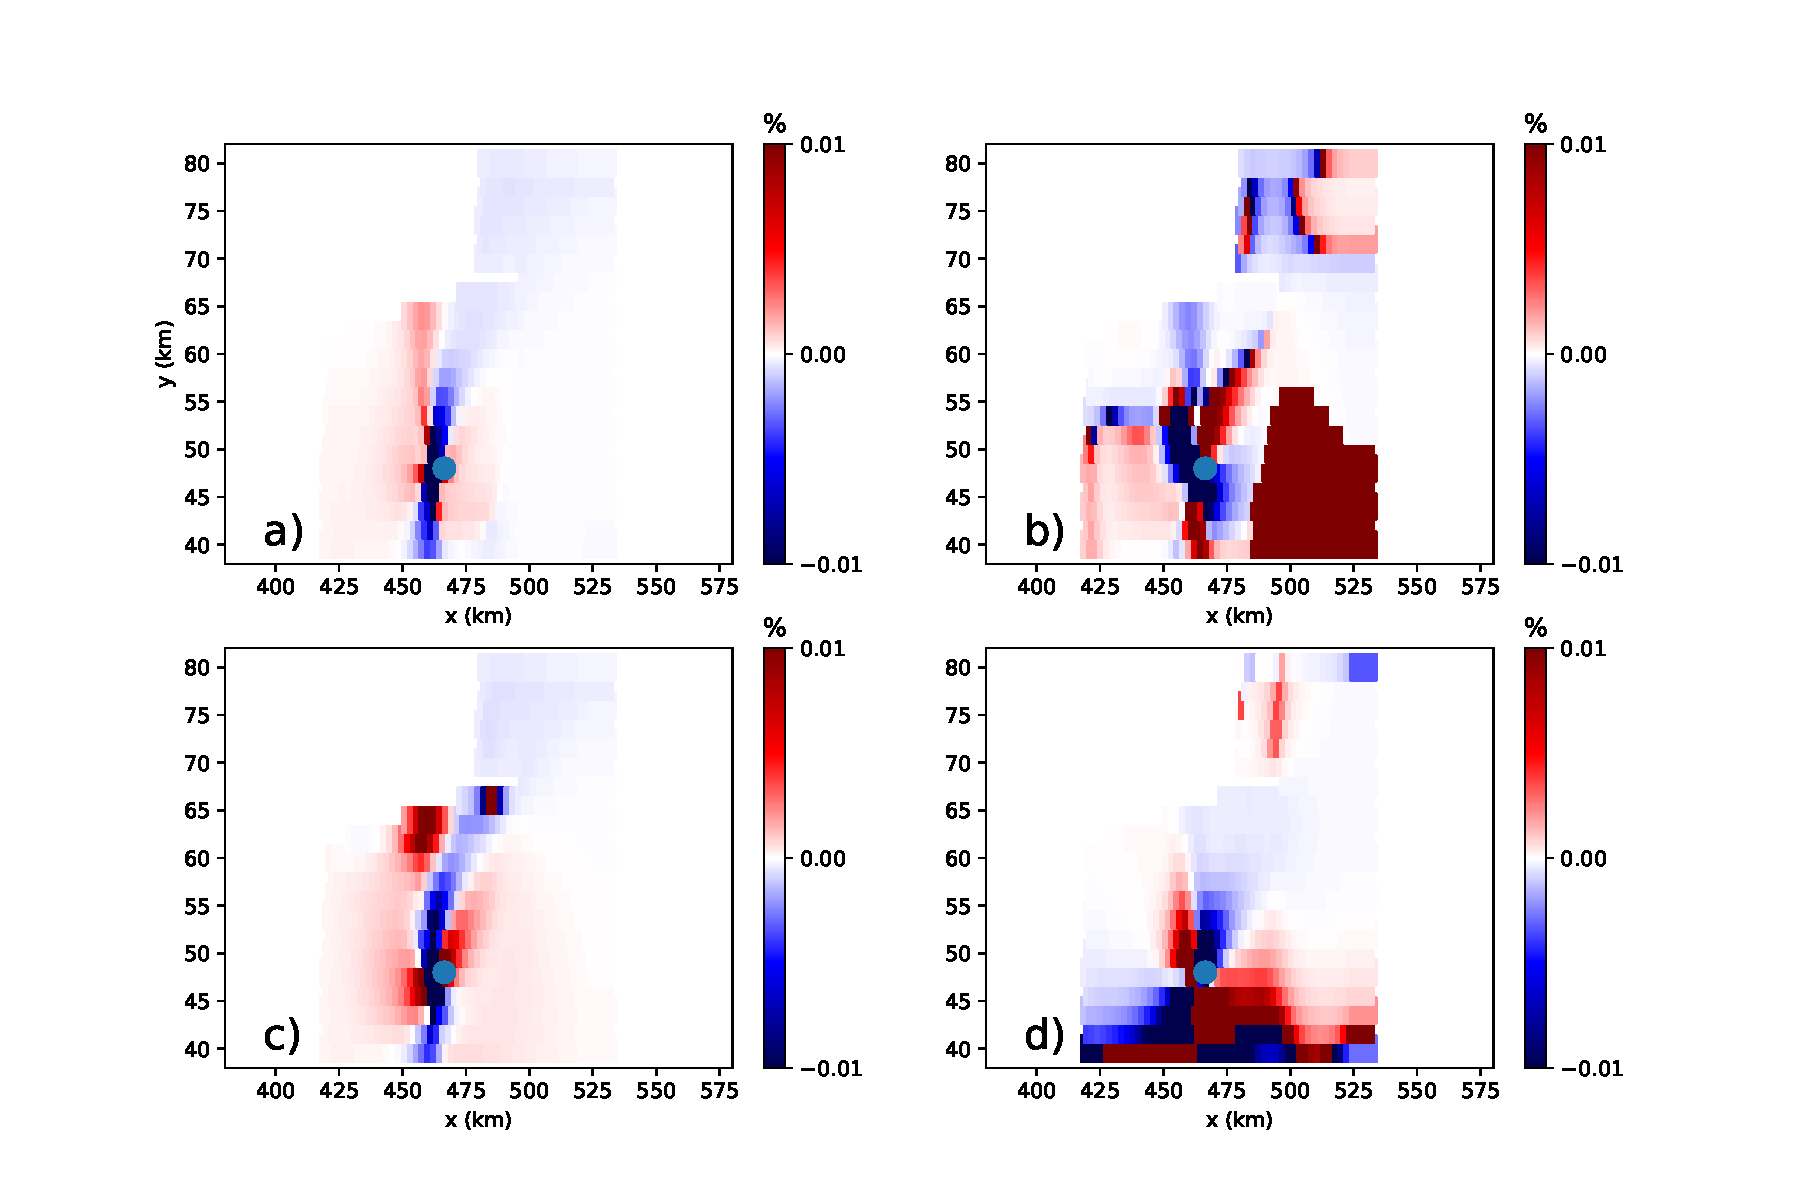
\includegraphics[width=1\linewidth]{figs/stressDiff.pdf}
%	\caption{An example of stress component changes (\%) across the MISMIP+ ice shelf and grounding line after apply the perturbations at different locations (blue circles). (a) Changes of $\sigma_{p1}$; (b) Changes of $\sigma_{p2}$; (c) Changes of $\sigma_{f}$; (d) Changes of $\sigma_{s}$;.}
%	\label{stressDiff}
%\end{figure}
%
%\begin{figure}
%	\centering
%	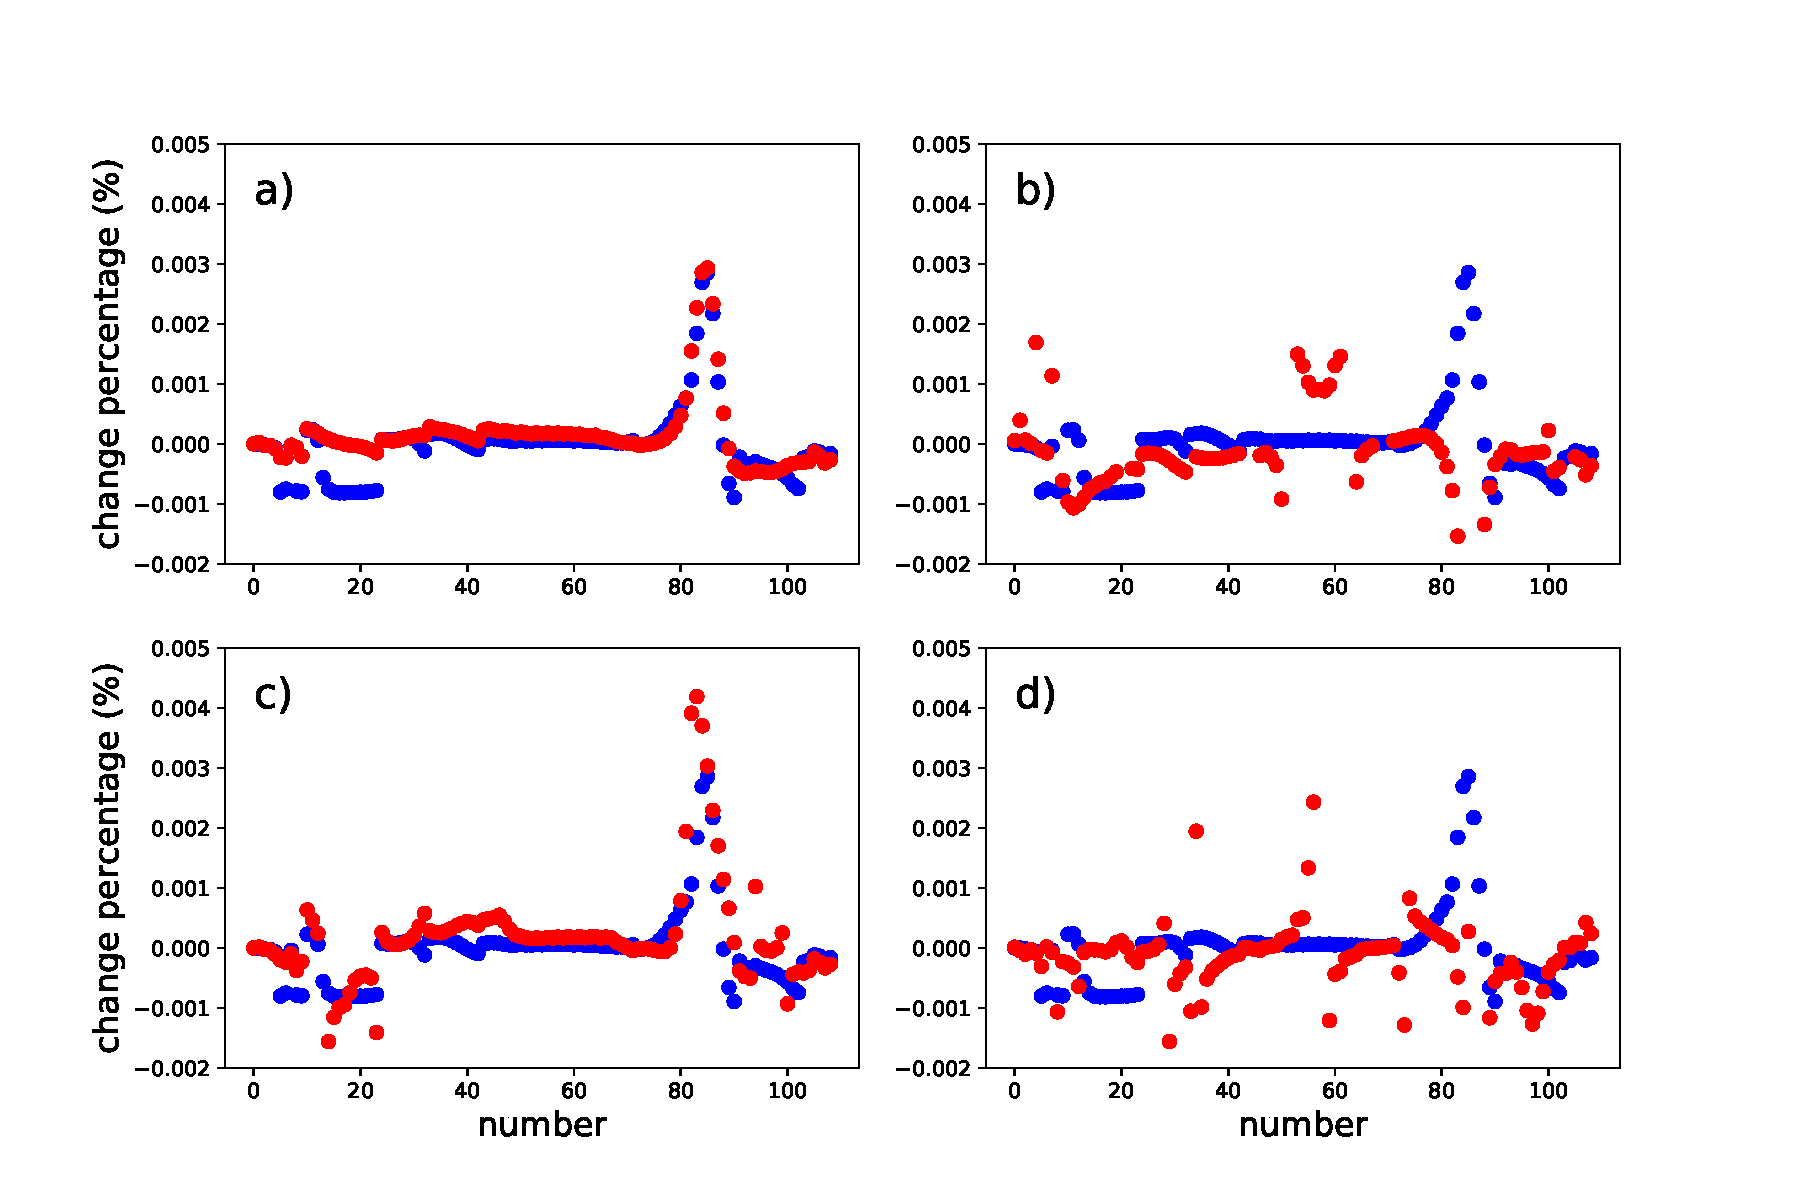
\includegraphics[width=1\linewidth]{figs/diffStress_diffVel.pdf}
%	\caption{The change percentage of ice speed (blue dots) and stress components (red dots; a--d represents $\sigma_{p1}$, $\sigma_{p2}$, $\sigma_{f}$ and $\sigma_{s}$, respectively) for all cells at the grounding line corresponding to Fig.~\ref{stressDiff}.}
%	\label{stressDiff_velDiff}
%\end{figure}

\end{document}
